\synctex=1
\documentclass[a4paper,10pt]{article}

%% TO-DO: Achim and Schill in acknowl
%% TO-DO: link to repo in paper and suppl mat
%% TO-DO: my new grant
%% TO-DO: give URLs to, e.g, Crooks reference: mybibwithurl?

%% For tracking changes
%% https://tex.stackexchange.com/questions/65453/track-changes-in-latex

% packages


% %% txfonts breaks amsmath.
% %% http://www.texfaq.org/FAQ-alreadydef

\usepackage{gitinfo2}

\usepackage{savesym}
\usepackage{amsmath}
\savesymbol{iint}
\usepackage{txfonts}
\restoresymbol{TXF}{iint}

\usepackage[utf8]{inputenc} % allows usage of spanish special characters
\usepackage[spanish,english]{babel} % english dictionary for proper hyphenation
%\usepackage{txfonts} % nice fonts
\usepackage{authblk} % author affiliations
\usepackage{graphicx} % images
\usepackage{float} % image positioning
\usepackage{subcaption} % collages of multiple images
%%\usepackage[hidelinks]{hyperref} % hyperlinks
\usepackage{hyperref}
% \usepackage{cite} % contraction of references, use
%                   % \usepackage[superscript]{cite} for superscript
%                   % citations
%% cite does not follow the usual pre and post citation
\usepackage[square,numbers,sort&compress]{natbib}
\usepackage{xcolor} % text color
\usepackage[margin=3cm]{geometry} % margins
\usepackage{lineno} % line numbers
\usepackage{csquotes} % paragraph quotes
\usepackage{multirow} % joining rows in tables
\usepackage{array}
\usepackage[normalem]{ulem}
\usepackage{todonotes}
%%\usepackage{amsmath}: something breaks. What?
\usepackage{pdflscape} %% Landscape
\usepackage{ulem} % strike-through text

%% cross references with suppl mat
\usepackage{nameref}
\usepackage{zref-xr,zref-user}
\zxrsetup{toltxlabel}
\zexternaldocument*[S-]{supp}
\hypersetup{
  colorlinks = true,
  citecolor=  black,
  linkcolor = {blue},
  filecolor = cyan %% controls color of external ref, if used
}



% customization
\setcounter{Maxaffil}{0} % affiliations
\renewcommand\Affilfont{\itshape\small} % style of affiliations text
\captionsetup[figure]{font=small, labelfont={bf}, labelformat={default}, labelsep=period, name={Fig.}} % custom figure captions
\makeatletter\renewcommand{\@biblabel}[1]{#1.}\makeatother % change [number] for number. in reference list
\newcommand{\idea}[1]{\textcolor{red}{#1}}
\newcommand{\mr}{\textcolor{red}{\textbf{[missing ref(s)]}}}
\newcommand{\change}[2]{\textcolor{red}{\sout{#1}}\textcolor{blue}{#2}}
\linenumbers % add line numbers to whole doc

% title, authors, affiliations
\title{Conditional prediction of consecutive tumor evolution using cancer
  progression models: What genotype comes next?}
%\title{Conditional prediction of short-term tumor evolution using cancer progression models}
%\title{Prediction of consecutive tumor evolution using cancer progression models}
%\title{Conditional prediction of upcoming tumor evolution using cancer progression models}
%\title{Partial prediction of tumor evolutionary trajectories using cancer progression models}
%\title{Using cancer progression models to predict upcoming tumor evolution}
\author[1,2,3]{Juan Diaz-Colunga}
\author[1,2,$\dagger$]{Ramon Diaz-Uriarte}
\affil[1]{Dpt. of Biochemistry, School of Medicine, Universidad Autónoma de Madrid, Madrid, Spain}
\affil[2]{Instituto de Investigaciones Biomédicas `Alberto Sols'
  (UAM-CSIC), Madrid, Spain}
\affil[3]{Department of Ecology \& Evolutionary Biology and Microbial
  Sciences Institute, Yale University, New Haven, CT, USA}
%\affil[3]{Dpt. of Ecology and Evolutionary Biology, Yale University, New Haven, Connecticut, USA}
%\affil[4]{Microbial Sciences Institute, Yale University, New Haven, Connecticut, USA}
\affil[$\dagger$]{To whom correspondence should be addressed: \normalfont ramon.diaz@iib.uam.es}
%\date{}

\begin{document}


% \date{\gitAuthorDate\ {\footnotesize (Release\gitRels: Rev:
%      \gitAbbrevHash)}}

\maketitle

\begin{abstract}

  Accurate prediction of tumor progression is key for adaptive
  therapy and precision medicine. Cancer progression models (CPMs) can be
  used to infer dependencies in mutation accumulation from cross-sectional
  data and provide predictions of tumor progression paths. But their
  performance when predicting the complete evolutionary paths is limited
  by violations of assumptions and the size of available data
  sets. Instead of predicting full tumor progression paths, we can focus
  on short-term predictions, more relevant for diagnostic and therapeutic
  purposes. Here we examine if five distinct CPMs can be used to answer
  the question ``Given that a genotype with $\mathrm{n}$ mutations has
  been observed, what genotype with $\mathrm{n}+1$ mutations is next in
  the path of tumor progression'' or, shortly, ``What genotype comes
  next''. Using simulated data we find that under specific combinations of
  genotype and fitness landscape characteristics CPMs can provide
  predictions of short-term evolution that closely match the true
  probabilities, and that some genotype characteristics (fitness and
  probability of being a local fitness maximum) can be much more relevant
  than global features. Thus, CPMs can provide short-term predictions even
  when global, long-term predictions are not possible because fitness
  landscape- and evolutionary model-specific assumptions are violated.
  When good performance is possible, we observe significant variation in
  the quality of predictions of different methods. Genotype-specific and
  global fitness landscape characteristics are required to determine which
  method provides best results in each case.  Application of these methods
  to 25 cancer data sets shows that their use is hampered by lack of the
  information needed to make principled decisions about method choice and
  what predictions to trust. Fruitful use of these methods for short-term
  predictions requires adapting method's use to local genotype
  characteristics and obtaining reliable indicators of performance; it
  will also be necessary to clarify the interpretation of the method's results
  when key assumptions do not hold.
  
\end{abstract}

%% bioniformatics:  A maximum of 150 words is recommended. https://academic.oup.com/bioinformatics/pages/instructions_for_authors
%% PLoS Comp Biol: I think around 300




%% Length of ms: For bioinformatics: Original papers: up to 7 pages, this
%% is approx. 5000 words, not including figures,
%%
%% Do as pdftotext draft.pdf - | wc -w
%% Maybe rm refs and figures before word counting
%% Place \end{document} before refs; uncomment it.


%% As of now, this is twice as long as it should be for Bioinformatics:
%% 9400 words withouth figures.

\section{Introduction}\label{sec:intro}



Accurately predicting tumor evolution would allow for better prognosis and
treatment. Unfortunately, the stochastic components in key factors that
govern tumor progression (mutation, genetic drift or clonal selection
\cite{greaves_evolutionary_2015,lipinski_cancer_2016,williams2018}, as
well as non-genetic variability \cite{Brock2009} and the tumor
microenvironment \cite{Albini2007}) fundamentally limit
predictability. This is also common to other problems
\cite{lassig_predicting_2017, losos2018} such as the evolution of
antibiotic resistance \cite{toprak2012} or virulence \cite{Day2004}, where
even small increases in predictive power could be of critical importance
for the design of treatment strategies \cite{palmer2013}.


% what are cancer progression models?
Cross-sectional high-throughput data are widely available for many cancer
types, and Cancer Progression Models (CPMs) \cite{Beerenwinkel2014,
  beerenwinkel_computational_2016}, originally developed to identify
restrictions in the order of accumulation of mutations in tumors
using cross-sectional data, could thus be key tools for predicting cancer
progression. CPMs (implicitly) encode all the possible mutational
trajectories that are compatible with the restrictions and, for some
methods, provide probabilities of different paths (figure
\ref{fig:fig1}A-B). However their performance to infer the complete
evolutionary trajectories, from the root genotype with no driver mutations
to a final, fixated genotype, is limited
\cite{diaz-uriarte2019a,hosseini2019a}; this has been attributed mainly to
violations of the underlying assumptions of the models (fitness landscapes
with a single fitness maximum in the genotype with all loci mutated,
strong selection week mutation regime \cite{gillespie1983}) and the
difficulty to acquire
large, unbiased data sets to power them \cite{diaz-uriarte2019a}.



Predicting the complete evolutionary path, however, might not be the most
relevant objective. Detection of a specific tumor composition at a given
point in time automatically discards all mutational pathways that do not
visit the observed state, reducing the amount of possible evolutionary
trajectories that can be followed from then on and thus potentially
facilitating the task of predicting further tumor progression. In this
work we address the question of how accurately CPMs can predict short-term
cancer evolution after a genotype is detected: what is the state that
comes consecutively after or ``what genotype comes next''. Even if the
predictability of the complete path is low because of violations of method
assumptions, genotype-specific features could lead to local improvements
in short-term predictability \cite{bank_predictability_2016,
  visser2018,ferretti2018}. Moreover, in contrast to the more general,
non-local descriptors, these genotype-specific factors can provide more
detailed insight regarding the requirements for the methods to be
reliable. In fact, conditional predictions on the observed genotype are
arguably much more relevant than complete evolutionary path predictions
for both adaptive therapy \cite[e.g.,][]{melnikov2020,hansen2020a,
  stankova2019a} and for SMART (sequential, multiple assignment,
randomized trial) designs in dynamic treatment regimes for personalized
medicine \cite{tsiatis2020,chakraborty2013}.



[Fig.~\ref{fig:fig1} about here]

% Rather than analyzing full evolutionary
% trajectories, as has been done in other work
% \cite{diaz-uriarte2019a,hosseini2019a}, we focus here on the question
% ``what genotype comes next'', the partial paths from an observed tumor
% state to the state that comes consecutively after.


% This might, on the one hand, lead to improvements in predictive power,
% even when the predictability of the complete path is low because of
% violations of method assumptions: genotype-specific features could lead to
% local improvements in short-term predictability
% \cite{bank_predictability_2016, visser2018,ferretti2018}. On the other
% hand, conditional predictions on the observed genotype are much more
% relevant clinically and for treatment purposes in adaptive therapy
% \cite[e.g.,][]{melnikov2020,hansen2020a, stankova2019a} and for SMART
% (sequential, multiple assignment, randomized trial) designs in dynamic
% treatment regimes for personalized medicine
% \cite{tsiatis2020,chakraborty2013}.

% , accurately predicting the next genotype could be among
% the tools for the physician to become, in a game theory context, the
% ``rational leader'' that anticipates and steers to limit cancer's
% resistance strategies \cite{stankova2019a}; moreover, observed genotypes
% and predicted next genotypes could be of use in SMART (sequential,
% multiple assignment, randomized trial) designs in dynamic treatment
% regimes for personalized medicine \cite{tsiatis2020,chakraborty2013}.

% \cite[prenote][posnote]{hansen2020a}

% accurately predicting the
% next genotype would play a key role in adaptive therapy
% \cite[e.g.,][]{melnikov2020, hansen2020a,stankova2019a}, as ``(...) the
% ability to anticipate subsequent cancer cell responses, provides a
% critical opportunity to obtain more favorable outcomes by steering and/or
% limiting the cancer cell’s resistance strategies'' \cite[]




% are used in adaptive therapy \cite{whatever}

% form basis of SMART designs in individualized therapy
% could be used in SMART designs \cite{whatever---los dos libros}
% \cite{tsiatis2020,chakraborty2013}
% (yo: check los dos zotero dirs, and look for conditional on genotypes)

% \cite{melnikov2020}: inhibiting growth in bacteria

% \cite{hansen2020a}: adaptive therapy and cpompetitive supression: gral ref

% \cite{gluzman2020}: conditional treatment

% \cite{west2019}

% Motivated by the idea that information on the prospective advance of the
% disease, even if limited, can be of critical importance for the design of
% treatment strategies and can improve therapeutic outcomes
% \cite[p.~243i]{palmer2013}


% Information on the prospective advance of the disease, even if limited,
% can be of critical importance for the design of treatment strategies
% \idea{references, as in paper with Claudia}. \todo{YES! DO!}
% \idea{[Relate predicting next genotype to adaptive therapy ---tarea para
%   Ramon]}.



% Tumor progression is governed by a combination of factors such as mutation, genetic drift or clonal selection
% \cite{greaves_evolutionary_20152015,lipinski_cancer_2016,williams2018}, as well as non-genetic
% variability \cite{Brock2009} and the tumor microenvironment
% \cite{Albini2007}. These have important stochastic components that
% fundamentally limit predictability. The ability
% to understand and predict evolutionary dynamics in cancer would allow for
% better prognosis and treatment. Investigating the mutational profiles of
% evolving clones within a tumor is possible by means of high-throughput
% genome sequencing, but the use of accurate models of tumor evolution is
% still required to unveil the true paths of cancer progression
% \cite{McPherson2017}. This is not of exclusive relevance to cancer but
% also to problems such as the evolution of antibiotic resistance
% \cite{toprak2012} or virulence \cite{Day2004}.



% % what are cancer progression models?
% Cancer Progression Models (CPMs) identify restrictions in the order of
% accumulation of mutations within a tumor using cross-sectional data. They
% encode all the possible mutational trajectories that are compatible with
% the restrictions (figure \ref{fig:fig1}A-B), which can serve to narrow the
% search for the true distribution of tumor progression pathways. However
% their performance to infer these complete evolutionary trajectories, from
% the root genotype with no driver mutations to a final, fixated genotype,
% is limited \cite{diaz-uriarte2019a,hosseini2019a}; this has been
% attributed to various factors, such as violations of the underlying
% assumptions of the models and the difficulty to acquire large, unbiased
% data sets to power them \cite{diaz-uriarte2019a}.

% what are we studying?
% In practice, cancer can only be first detected once it has already
% advanced to some extent.


% Detection of a specific tumor composition at a given point in time
% automatically discards all mutational pathways that do not visit the
% observed state, reducing the amount of possible evolutionary trajectories
% that can be followed from then on and thus potentially facilitating the
% task of predicting further tumor progression.\todo{is it here where we
%   explain how this differs from work with Claudia?} In this work we
% address the question of how accurately CPMs can predict short-term cancer
% evolution after detection. Rather than analyzing full evolutionary
% trajectories, we focus on the partial paths from an observed tumor state
% to the state that comes consecutively after.



The question of what genotype comes next, or what is the state that comes
consecutively after, requires that we carefully define the meaning of
``consecutive'' states in this context. If cancer progresses under
conditions of strong selection and weak mutation (SSWM)
\cite{gillespie1983}, only evolutionary trajectories of increasing fitness
are possible, and the evolution of a new, higher-fitness clone results in
rapid expansion and effective exclusion of previous ones before any new
mutations take place. In this situation, there is a well defined sequence
of genotypes with progressively increasing fitness in the path to tumor
fixation, with the most abundant clone at every time being a direct
descendant of a previously most abundant one itself (figure
\ref{fig:fig1}C). But, in cancer, large population sizes and high mutation
rates can prevent successful clonal sweeps \cite{nichol2019a, zhao2016} so
that instead of SSWM, clonal interference and stochastic tunneling
\cite{devisser_empirical_2014,szendro_predictability_2013,sniegowski_beneficial_2010,
  wodarz_dynamics_2014} become common: multiple clones can coexist at
significant fractions for prolonged periods of time, and new
higher-fitness clones can evolve from low fitness parents that represented
a minority of the population
(Fig~\ref{fig:fig1}D). % As a consequence, genotypes with a large
% number of mutations %high mutational load
% can already be present at the time of sampling yet go undetected if their
% relative abundance is small (figure
% \ref{fig:fig1}D). % Deviations from SSWM
% are known to undermine the predictive power of CPMs
% \cite{diaz-uriarte2018,diaz-uriarte2019a}, as the model underlying most
% CPMs seems to assume SSWM (see Discussion). This assumption, however, is
% not always stated
% explicitly.
% , but it is explicit, for example, in Hosseini et al.'s
% \cite{hosseini2019a} use of CPMs for predicting tumor evolution (see
% \nameref{discussion}).






To formulate the question of ``what genotype comes next'' 
%To accurately raise a question that does not rely on SSWM to be well
%defined,
so that it does not depend on the SSWM assumption we designate an
\textit{observed} genotype as that which is most abundant in the tumor at
the time of sampling. On the other hand, a Line of Descent (LOD) is
defined as a sequence of parent-child genotypes from the wild-type to the
(possibly local) 
fitness maximum where fixation occurs \cite{szendro_predictability_2013}.
By construction, assuming that mutations accumulate one by one and cannot
be lost, each genotype in the LOD has all the mutations of the previous
one plus exactly one more (as it directly descends from it). The LOD has
no more than one genotype with a given number of mutations, whereas in
general two or more observable genotypes could share the same mutation
count (e.g. in figure \ref{fig:fig1}D both the red and green genotypes
have one mutated driver and are observable). If the evolutionary process
does not conform to SSWM, not all genotypes in the LOD are necessarily
observable. From a clinical perspective, it is relevant to use the
information that is detectable to unveil the underlying dynamics of cancer
evolution, encoded in the LOD. In other words, we want to make a
prediction regarding \textit{what comes next in the LOD} based on the
\textit{observation} of a genotype. We thus formulate the following
general question: \textit{Given that a genotype with $\mathrm{n}$
  mutations has been observed, what genotype with $\mathrm{n}+1$ mutations
  is in the LOD?} Formulated like this, the question is unambiguous and
determined. Under SSWM conditions it can be expressed simply as:
\textit{given that a certain genotype has been observed, what genotype
  comes next in the path to tumor fixation?} However, it is important to
emphasize that even if there is no SSWM the more general question remains
well defined.

% how do we do it?

To address this question, we use a collection of evolutionary simulations
from which we obtain the true paths of tumor progression. For every
simulated process we keep track of % what genotypes represent the majority
% of the population as the tumor progressed (i.e., we list 
the most frequent genotypes. Then for each one of them we ask what
genotype has exactly one more mutation while also being a direct ancestor
of the ultimately fixated clone. Averaging over all simulations we obtain
a set of frequencies which represent the conditional probabilities that we
are interested in. We then examine five CPMs: Mutual Hazard Networks (MHN)
\cite{schill2020}, Conjunctive Bayesian Networks (CBN)
\cite{Gerstung2009,Gerstung2011,montazeri_large-scale_2016}, Oncogenetic
Trees (OT) \cite{Desper1999JCB,Szabo2008}, CAncer PRogression Inference
(CAPRI) \cite{capri_bioinformatics,capri_pnas} and CAncer PRogression
Extraction with Single Edges (CAPRESE) \cite{caprese_2014}, some of which
have more than one variant (giving a total of 13 different methods). We
provide these methods with cross-sectional samples taken from the
evolutionary simulations and compare their predictions with the true
probabilities. We explore the factors that affect performance, focusing on
those factors that depend on the properties of the observed genotype. We
want to understand whether CPMs can be used to predict short-term
evolution; for this question, the key response variable is the best
possible performance over all CPMs considered. Although we do address
method choice as a secondary question, this is not our main objective 
\textit{per se}. We discuss the consequences of our results for the analysis of
cancer data by analyzing 25 cancer data sets.


% This work differs from earlier work \cite{diaz-uriarte2019a,hosseini2019a}
% in that we examine a completely different question: previous work dealt
% with predicting full evolutionary trajectories, but here we examine the
% short-term prediction question \textit{Given that a genotype with
%   $\mathrm{n}$ mutations has been observed, what genotype with
%   $\mathrm{n}+1$ mutations is in the LOD?}, which can colloquially be
% summarized as ``What genotype comes next''. In addition, we add a recent
% new method, Mutual Hazard Networks (MHN) \cite{schill2020}, which is very
% different from the rest of the CPMs considered here. Moreover, we are
% examining genotype-specific factors in addition to global fitness
% landscape characteristics: in contrast to the more general, non-local
% descriptors that may not apply to the totality of the fitness
% landscape/evolutionary process, these genotype-specific factors can
% provide more detailed insight regarding the requirements for the methods
% to be reliable in what are arguably the more relevant questions for
% individualized and precision medicine.





% Why does this matter? Predicting important. In fact,

% experimental evolution studies in bacteria and yeast have allowed to
% partially disentangle the role of population size, selection, and
% mutational heterogeneity in parallel evolution \cite{bailey2017} and,
% thus, indirectly on the issues addressed here; using these results for
% cancer, however, would require much more detailed information (e.g.,
% effective population sizes) than is often available.

% So, what can we do with experimental data from cancer? This we examine in
% the discussion blablaba



% \idea{We probably need to make it explicit how it differs from previous
%   work, in particular Diaz-Uriarte and Vasallo.  If we end up doing what I
% think about comparing JS of methods and using that for real data sets, an
% additional comment is ``and we provide specific, practical advice that can
% be followed with the output of methods applied on real data'' ---or
% something of that sort}.
% \idea{Relate to this: Detection of a specific tumor composition at a given point in
% time automatically discards all mutational pathways that do not visit the
% observed state, reducing the amount of possible evolutionary trajectories
% that can be followed from then on and thus potentially facilitating the
% task of predicting further tumor progression. And relate to Bank}


% \idea{Say something about trying to identify, from method output itself,
%   when good performance}


% \idea{We use MHN. First to review that method. We use CPMs, but also
%   include MHN, a newly developed approach that blablab}


% \idea{This is KEY: we do what really matters: next genotype. It really
%   matters because: a) global predictions suck and are generally doomed
%   except maybe to estimate predictability; b) global predictions can
%   not benefit from local features; c) newxt is what matters for therapy
%   and adaptive treatment}.


\section{Methods} \label{methods}

\subsection{Overview}
\label{sec:overview}

To assess if we can use CPMs for short-term predictions of evolutionary
processes, we have compared predicted and true answers to the question
\textit{Given that a genotype with $\mathrm{n}$ mutations has been
  observed, what genotype with $\mathrm{n}+1$ mutations is in the LOD?}
under an extensive set of simulated scenarios. First, we simulated a large
number of tumor evolution trajectories under scenarios with varying
departures from the assumptions of CPM methods; next, we obtained a large
number of simulated tumor evolution trajectories.  Next, we emulated
cross-sectional sampling of the simulations, with varying sampling schemes
and sample sizes. These steps are described in section
\nameref{methods:simulsandsampling}.  The transition probabilities that
provide the true answer to the question \textit{Given that a genotype with
  $\mathrm{n}$ mutations has been observed, what genotype with
  $\mathrm{n}+1$ mutations is in the LOD?}  is explained in section
\nameref{sec:methods:sim}. To obtain the CPM predictions we analyzed each
of the sampled data sets with a total of 13 different CPM variants and
obtained the predictions as explained in section
\nameref{methods:cpm}. Next, we measured how close the predictions were to
the truth (section \nameref{sec:js}) and, finally, we analyzed the major
factors that affect the similarity between predictions and truth (section
\nameref{sec:linear-mixed-model}).  To examine the implications of our
results for the analyses of cancer data, we have analyzed 25 cancer data
sets, described in section \nameref{sec:datasets}.


\subsection{Simulated evolutionary processes and sampling} \label{methods:simulsandsampling}

Simulated data were taken from \cite{diaz-uriarte2019a}, where complete
details are provided. In summary, simulations were conducted under
evolutionary scenarios that differed in the number of genes, the type of
fitness landscape, the initial population size, and the mutation
rates. Landscapes were of either 7 or 10 genes. Fitness landscapes were of
three types: representable, local maxima or Rough Mount Fuji (RMF). The
three types of fitness landscapes incorporate increasing departures from
the assumptions of most CPMs: for the representable fitness landscapes a
DAG of restrictions exists with the same accessible genotypes and
accessible mutational paths; for local maxima fitness landscapes the set
of accessible genotypes can be represented by a DAG of restrictions, but
there are local fitness maxima and the fitness graph has missing paths
\cite{diaz-uriarte2019a}; the genotype with all genes mutated might or
might not be the genotype with largest fitness. The RMF fitness landscapes
\cite{neidhart_adaptation_2014, devisser_empirical_2014,fragata2019}
usually have multiple local fitness maxima and considerable reciprocal
sign epistasis so not even the set of accessible genotypes can be
represented by a DAG of restrictions. On the above fitness landscapes
evolutionary simulations were run. Three different populations sizes
($2\times10^3$, $5\times10^4$ or $1\times10^6$) and two mutation rate
regimes (mutation rate fixed at $10^{-5}$ or uniformly distributed in the
log scale between $0.2\times10^{-5}$ and $5\times10^{-5}$) were used to
generate variability with respect to SSWM. For each combination of the
above factors, 35 independent replicates were obtained for a total of 1260
landscapes (35 replicates $\times$ 2 number of genes $\times$ 3 types of
fitness landscapes $\times$ 3 initial population sizes $\times$ 2 mutation
rate regimes). Then, for each one of them, 20000 independent evolutionary
processes were simulated until fixation of one of the genotypes at a
fitness maximum (local or global). The complete history of the simulations
was stored so that the true LOD for each simulation was known. Each set of
simulations was then sampled under three detection regimes: with equal
probability with respect to the size distribution (\textit{uniform}
sampling), sampling predominantly early in the tumor progression process
(i.e., enriched in \textit{small} tumors), sampling predominantly late in
the tumor progression process (i.e., enriched in \textit{large}
tumors). When \textit{sampling}, we identified the most abundant genotype
and its mutated loci at the chosen time, so the sampling process is
consistent with how we defined \textit{observable} genotypes earlier. No
sampling error is considered. The full sample consists of three binary
matrices of observations (one per detection regime), each with 20000 rows
(one observation per simulation) and as many columns as driver genes. Each
element of the matrix is either 1 or 0 (true or false) depending on which
genes were mutated in which observations. For each detection regime, the
complete sample was used to generate five smaller, non-overlapping splits
of size 50, 200 or 4000. This produced a total of 56700 data sets (1260
fitness landscapes $\times$ 3 detection regimes $\times$ 3 sample sizes
$\times$ 5 splits).

\subsection{Transition probabilities from evolutionary simulations}
\label{sec:methods:sim}

Let us consider a matrix $\mathbf{P}$ where rows correspond to observable
genotypes and columns to genotypes of the LOD. The element $(i,j)$ of the
matrix, denoted as $p_{ij}$, represents the conditional probability that
the genotype $j$ (with $n+1$ mutations) is an element of the LOD given the
genotype $i$ (with $n$ mutations) has been observed. In the absence of
back mutations and when mutations accumulate one by one, $p_{ij}$ is
defined only if $i$ and $j$ are exactly one mutation away from each other.
Note that the genotype $j$ (element of the LOD and with $n+1$ mutations)
need not be a direct descendant of $i$ if SSWM does not hold. We built a
transition matrix $\mathbf{P}$ for every fitness landscape that we
generated by examining each of the 20000 evolutionary processes that were
simulated in the corresponding landscape, listing all observable genotypes
(i.e. those that represented the majority of the population at some point
during the simulated evolutionary process) and extracting the LOD of every
process tracking back the ancestors of the fixated genotype (definition
and details in \cite{szendro_predictability_2013}; using implementation in
\cite{diaz-uriarte2017}).  Each element $p_{ij}$ can thus be interpreted
as the fraction of the times that $j$ was in the LOD given that an
observation of $i$ had been made. See further details in Supplementary
Material, section \ref{S-supp-cpm-details}.



% \subsubsection{Special cases}\label{sec:special}

% When the end of the evolutionary process is reached there are no further
% transitions to genotypes of the LOD. Thus, matrix $\mathbf{P}$, which
% provides the true probability distributions for the question \textit{what
%   genotype of the LOD has $\mathrm{n}+1$ mutations iven that a genotype
%   with n mutations has been observed?} needs to add to additional states
% that correspond to two distinct special cases. When the observed genotype
% is the final, fixated one, we have simply reached the end of the
% evolutionary process; we handle this by adding to the $\mathbf{P}$ an
% ``end" situation (denoted as $p_{i,end}$). If SSWM conditions are not
% satisfied, however, observable genotypes need not be a part of the LOD so
% that there could be observable genotypes with more mutated loci than, or
% as many mutated loci as, the final genotype that gets fixated. In other
% words, it is possible that a clone with $m \geq n$ mutations establishes
% in the tumor for a period of time even if eventually another clone with
% $n$ mutations is the one that fixates.  We handle this by adding to the
% $\mathbf{P}$ a ``none" situation ($p_{i,none}$). Downstream analyses are
% performed including these two probabilities ($p_{i,end}, p_{i, none}$)
% (and row normalization was actually carried out after including $end$ and
% $none$).


% % \subsection{Transition probabilities from evolutionary simulations}
% % \label{methods:sim}

% % Let us consider a matrix $\mathbf{P}$ where rows correspond to observable
% % genotypes and columns to genotypes of the LOD. The element $(i,j)$ of the
% % matrix, denoted as $p_{ij}$, represents the conditional probability that
% % the genotype $j$ (with $n+1$ mutations) is an element of the LOD given the
% % genotype $i$ (with $n$ mutations) has been observed. Naturally, $p_{ij}$
% % is defined only if $i$ and $j$ are exactly one mutation away from each
% % other. Note that, given how our question is formulated, all the mutations
% % in $i$ need to also be present in $j$ only in SSWM, when $i$ would
% % necessarily be the parent of $j$. But in a more general scenario (e.g.,
% % when SSWM does not hold) it is possible that a genotype $i$ with $n$
% % mutations is observed despite not belonging to the LOD. Therefore the
% % genotype $j$ (element of the LOD and with $n+1$ mutations) need not be a
% % direct descendant of $i$. The only condition for $p_{ij}$ to be defined is
% % that $j$ has exactly one more mutation than $i$:

% % \begin{equation}
% % p_{ij} \in \mathbb{R} \iff n_{mut}(j) = n_{mut}(i) + 1
% % \label{eq:pij}
% % \end{equation} 
% % \idea{En realidad, no es $\mathbb{R}$; es $[0, 1]$, puesto que podemos
% %   definirlo como 0. }



% % We built a matrix $\mathbf{P}$ for every fitness landscape that we
% % generated. To obtain the elements $p_{ij}$ of one of them, we ran through
% % all 20000 evolutionary processes that were simulated in the corresponding
% % landscape. In each case, we first listed all observable genotypes
% % (i.e. those that represented the majority of the population at some point
% % during the simulated evolutionary process). Then we extracted the LOD of
% % every process tracking back the ancestors of the fixated
% % genotype (see definition and details in \cite{szendro_predictability_2013}; using implementation in \cite{diaz-uriarte2017}).
% % We identified the genotypes in the LOD with one mutation more than the
% % observable ones, and added 1 to the corresponding entries of
% % $\mathbf{P}$. Finally, we row-normalized $\mathbf{P}$ to meet the
% % normalization condition $\sum_{j} p_{ij} = 1$.

% % % \begin{equation}
% % % \sum_{j} p_{ij} = 1
% % % \label{eq:pij-norm}
% % % \end{equation}\todo{Added this equation, OK?}
% % %
% % Each element $p_{ij}$ can thus be interpreted as the fraction of the times that $j$ was in the LOD given that an observation of $i$ had been made. For a large number of simulations, this fraction represents a good approximation of the true probabilities.

% % \subsubsection{Special cases}\label{sec:special}


% % If SSWM conditions are not satisfied, observable genotypes need not be a part of the LOD and not all genotypes in the LOD are necessarily observable. A particular case of this are observable genotypes with more mutated loci (or just as many) than the final one that gets fixated: it is possible that a clone with $m \geq n$ mutations establishes in the tumor for a period of time even if eventually another clone with $n$ mutations is the one that fixates. This represents a special scenario for our purpose: the answer to out question (\textit{what genotype of the LOD has $\mathrm{n}+1$ mutations?}) is technically undefined if the LOD stops at $n$ mutations. We identify two scenarios: \textit{a)} the observed genotype is simply the final, fixated one, and \textit{b)} the observed genotype has transiently established as the most abundant, but fixation will occur at a different one (with less mutations) evolving through a different pathway.
% % \iffalse

% % \begin{itemize}
% % \item[\textit{a)}] The observed genotype is simply the final, fixated one.
% % \item[\textit{b)}] The observed genotype has transiently established as the most abundant, but fixation will occur at a different one (with less mutations) evolving through a different pathway.
% % \end{itemize}
% % %
% % \fi
% % We refer to \textit{a)} as an ``end" situation (we have simply reached the end of the evolutionary process), and to \textit{b)} as a ``none" situation (the only possible answer to our question is ``there is no such a genotype"). In practice, we handle these cases by attaching two additional columns to $\mathbf{P}$. These contain the probabilities that an observation of a genotype $i$ is made in an ``end" situation (denoted as $p_{i,end}$) or a ``none" situation ($p_{i,none}$). Downstream analyses are performed including these probabilities.

% % \idea{[Move all this chunk (or even almost everything after \ref{eq:pij})
% %   to the Supplementary? I'm worried it may break the flow of the
% %   paper. Would it make sense to simply write a super-simplified methods
% %   with just enough information to follow the reasoning, and move
% %   everything else to the supplementary?]}\todo{something needs to be left
% %   here, maybe all. Not sure yet how much, though}

\subsection{Transition probabilities from CPMs} \label{methods:cpm}

%  \idea{Explain how we go from the output of a CPM (DAG of restrictions,
%    but not in the time-discretized cases?)}\todo{in Diaz-Uriarte and
%    Vasallo (except we stop at the transition matrix between genotyps stage
%    ---I'll write it)}
% \idea{Notation: matrix of predictions from a CPM should be named
%   $\mathbf{\widehat{P}}$, and its elements $\hat{p}_{ij}$. The hat
%   indicates an estimator, which is precisely what CPMs provide: an
%   estimation of the true probabilities $p_{ij}$.}

General overviews of all the methods used here, except for MHN, are
available in \cite{beerenwinkel_computational_2016, Beerenwinkel2014,
  diaz-uriarte2019a,diaz-uriarte2018} and detailed descriptions are given
in the original references for each procedure (MHN \cite{schill2020}, CBN
\cite{Gerstung2009, Gerstung2011}, MCCBN
\cite{montazeri_large-scale_2016}, OT \cite{Szabo2008, Desper1999JCB},
CAPRI \cite{capri_bioinformatics, capri_pnas}, CAPRESE
\cite{caprese_2014}). Briefly, CBN, MCCBN, OT, CAPRESE, and CAPRI try to
identify restrictions in the order of accumulation of mutations from
cross-sectional data. CAPRESE and OT code these restrictions using trees
(i.e., under these two methods each event, such as a mutation, can
immediately depend on at most one other event); although the output of OT
and CAPRESE is often similar, the procedures are different (in OT weights
along edges can be directly interpreted as probabilities of transition
\cite{Szabo2008}, whereas CAPRESE uses a probability raising notion of
causation based on Suppes' probabilistic causation). CBN, MCCBN, and CAPRI
code these restrictions using DAGs (i.e., each event can depend on
multiple other events).  CBN and MCCBN are very closely related methods:
the CBN version we use is H-CBN as described in \cite{Gerstung2009,
  Gerstung2011}, and MCCBN is an implementation of the CBN model that uses
a Monte Carlo Expectation-Maximization (EM) algorithm for fitting the CBN
model \cite{montazeri_large-scale_2016} (instead of the simulated
annealing nested within EM of H-CBN); in contrast, CAPRI tries to identify
probability raising in the framework of Suppes' probabilistic
causation. Common to most of these methods is a model of deterministic
dependencies \cite{schill2020}, a model of accumulation of mutations where
an event (a mutation) can only occur if all its dependencies are satisfied
(though different methods allow for small error deviations from this
requirement); CAPRI and CAPRESE try to recover ``probability raising''
relations and, strictly, their trees/DAGs do not encode deterministic
dependencies but will be treated as doing so in this paper, since
obtaining probabilities of transition from them is not possible otherwise
---see details in section \nameref{S-supp-trans-prob} in the Supplementary
Material.

For all of these methods, since a DAG of restrictions determines a fitness
graph (see Fig.~\ref{fig:fig1} A-B and
\cite{diaz-uriarte2018,diaz-uriarte2019a}), we can obtain the set of
possible descendants for a genotype directly from this fitness graph.  For
CAPRESE and CAPRI all transitions were set as equiprobable (as
probabilities of transition are not available) but for CBN, MCCBN, and OT
we can compute the probabilities of transition between genotypes. CBN and
MCCBN return the parameters of the waiting time to occurrence of each
mutation given its restrictions are satisfied which allows us to compute
transition probabilities between genotypes using competing exponentials
(see \cite{montazeri_large-scale_2016, hosseini2019a, diaz-uriarte2019a})
and a similar procedure can be used with OT by using the edge weights
(though, strictly, the OT model, being an untimed oncogenetic tree does
not return these probabilities ---see \cite{diaz-uriarte2019a}). Mutual
Hazard Networks (MHN) \cite{schill2020} differ from the previous methods
in that events are modeled by a spontaneous rate of fixation and a
multiplicative effect each of these events can have on other events (i.e.,
pairwise interactions), which allows it to model both enabling and
inhibiting dependencies. The output of MHN is a transition rate matrix; as
for CBN and MCCBN, we can obtain the probability of transition to each
descendant genotype, given a transition, using competing exponentials from
the transition rate matrix (see equation 2 and Fig.~2 in
\cite{schill2020}). Details on software and computation of transition
probabilities are provided in the Supplementary Material, sections
\nameref{S-supp-cpm-details} and \nameref{S-supp-trans-prob}.


% \subsubsection{Time-discretized CPMs}\label{sec:td}

None of the CPM models considered here allow us to accommodate local
maxima: under all of the models, the genotype with all genes mutated is
always reached with probability 1 as time goes to infinity (this is also
the case for MHN, even if it can include inhibiting effects). To overcome
this limitation without making specific additional assumptions about the
sampling process, and for MHN, CBN, and MCCBN, we have used the
uniformization method \cite{grassmann1977,vandijk2018} (see also
\cite[Fig.\ 6]{schill2020}) to approximate the continuous-time Markov
chain ($\mathbf{Q}$) by a discrete time Markov chain 
(with transition matrix $= \mathbf{I} + \frac{1}{\gamma}\mathbf{Q}$, where
$\gamma = \max(|q_{ii}|)$). We will interpret the diagonal entries of the
time-discretized transition matrix as a lower bound on the probability
that the given genotypes behave as local maxima. The output from CBN, MHN,
and MCCBN after time discretization will be referred to as CBN\_td,
MHN\_td, and MCCBN\_td, respectively, and we will differentiate this
\textbf{time-discretized} results from those obtained, as explained above,
using competing exponentials. We will refer to these methods as the
\textbf{TD} methods (for time-discretized) whereas their counterparts,
CBN, MHN, MCCBN, obtained via competing exponentials on the rate
matrix, woll be referred below as the CE methods. OT, CAPRESE, and CAPRI do not
belong to any of those two groups, though none of them can accommodate
local maxima either; thus, when we refer to the ``non-TD'' methods, that
includes MHN, CBN, MCCBN (in their ``non-TD'' versions) as well as OT,
CAPRESE, and CAPRI.
%%CEr
%(``CE'' in Figure \ref{fig_biol_comp}).


% \idea{We should justify that much better. I don't see how. And first
%   sentence is the same as saying that the limiting distribution is
%   $\pi_{gentoypeWithAllGenesMutated} = 1$. Not sure that clarifies things
% for most readers.} 


In summary, a total of 13 methods have been used: CBN, in three variants
(CBN, with transition probabilities using competing exponentials
conditional on transition; CBN\_uw, obtained from the former by using
equiprobable transitions; CBN\_td, the time-discretized version of CBN);
MCCBN, again in three variants (MCCBN; MCCBN\_uw; MCCBN\_td);
MHN in two variants (MHN and MHN\_td); OT in variants OT and OT\_uw
(equiprobable transitions); CAPRESE; CAPRI, in two variants, CAPRI\_AIC,
CAPRI\_BIC (which differ on the penalty used, AIC or BIC). Each of these
methods returns a matrix $\mathbf{\hat{P}}$ of predicted transition
probabilities. 






% \idea{MHN: give a few details of how we used it. Basically, default with
%   parameters for balbla}\todo{explain something about the All others too?
%   CBN, OT, etc? It will
% be the fourth time I do it! Or refer to previous papers and just add a
% sentence for MHN? -- I would definitely just add the references, maybe a short general explanation of "traditional" CPMs and then add a couple more sentences for MHN (and maybe time-discretized versions of CBN and MCCBN)}


% \idea{misra: discuss how it is similar or different. Or in the intro. Or
%   in the methods. Who cites Misra?. Misra looks similar, but it gives a
%   0/1 decision, and has a parameter, threshold, `` (any number between 0
%   and 1), smaller numbers give you more detail (give a number between 0
%   and 1 that specifies the level of detail in output path file, this file
%   will have a .dot extension. We used 0.3 in the manuscript)'' And Misra
%   seems to only find ancestor of existing genotypes. So genotypes that are
%   not present (at least with many mutations) are never predicted to
%   exist. It is a somewhat different method, with difficult to use code,
%   and poorly explained arguments. Its output are not really probabilities
%   of paths.  }




\subsection{Quantification of similarity between predicted and true
  transition probabilities} \label{sec:js}

For every observed genotype $i$ we have compared the vector of true
probabilities $\mathbf{p}_i$, from the $i$th row of $\mathbf{P}$ with the
analogous vector of predictions from a CPM $\mathbf{\hat{p}}_i$ returned
from the $i$th row of $\mathbf{\hat{P}}$ for each CPM. We measured the
similarity between these two vectors using the Jensen-Shannon distance
($JS$) \cite{crooks2017}, the square root of the Jensen-Shannon divergence
\cite{lin1991}. The Jensen-Shannon divergence is a symmetrized
Kullback-Leibler divergence between two probability distributions that is
0 when the two distributions are identical and reaches its maximum value
of 1 if the two distributions do not overlap (we used log of base 2). See
further details in Supplementary Material, section \ref{S-supp-js}.



% Consider the vector of true probabilities
% $\mathbf{p}_i=\left(p_{ia},p_{ib},\cdots,p_{iz}\right)$, where
% $a,b,\cdots,z$ are all genotypes with one mutation more than $i$: this is
% nothing but the $i$-th row of the matrix $\mathbf{P}$ (excluding the
% elements that do not satisfy $n_{mut}(j) = n_{mut}(i) + 1$). Consider also
% the analogous vector of predictions from a CPM $\mathbf{\hat{p}}_i$. We
% measured the similarity between these two vectors using the Jensen-Shannon
% distance ($JS$) \cite{crooks2017}, the square root of the Jensen-Shannon
% divergence \cite{lin1991}. The Jensen-Shannon divergence is a symmetrized
% Kullback-Leibler divergence between two probability distributions that is
% 0 when the two distributions are identical and reaches its maximum value
% of 1 if the two distributions do not overlap (we used log of base 2); it
% is defined even if the two distributions do not have the same sample space
% (i.e., even if $p_i \ne 0$ and $q_i = 0$ or viceversa). (And the square
% root of the Jensen-Shannon divergence is a metric between probability
% distributions \cite{crooks2017})

% \idea{CHECK: ``excluding the undefined elements that do not satisfy the
%   condition in equation ref{eq:pij}'' : En realidad, no need to exclude
%   them; just set them to 0. This is equivalent. Pero dejo el ``excluding
%   the elements that do not satisfy $n_{mut}(j) = n_{mut}(i) + 1$'' que
%   juega el mismo papel}.





% Using the Jensen-Shannon distance, the square root
% of the Jensen-Shannon divergence is a metric between probability
% distributions.

% The Jensen-Shannon distance between them is defined as \cite{crooks2017, lin1991}.

% \begin{equation}
% JS\left(\mathbf{p}_i,\mathbf{\hat{p}}_i\right) = \sqrt{\frac{1}{2}d_{KL}\left(\mathbf{p}_i,\mathbf{q}\right) + \frac{1}{2}d_{KL}\left(\mathbf{\hat{p}}_i,\mathbf{q}\right)}
% \label{eq:js}
% \end{equation}
% %
% where we have used the Kullback–Leibler divergence, defined for two arbitrary vectors $\mathbf{x}=\left(x_1,x_2,\cdots\right)$ and $\mathbf{y}=\left(y_1,y_2,\cdots\right)$ as

% \begin{equation}
% d_{KL}\left(\mathbf{x},\mathbf{y}\right) = \sum_i x_i \log_2 \frac{x_i}{y_i}
% \label{eq:kl}
% \end{equation}
% %
% $JS$ is bounded between 0 and 1, is minimal when $\mathbf{p}_i$ and
% $\mathbf{\hat{p}}_i$ are identical and largest when they are maximally
% different. \idea{We opted for this metric because... and it is defined
%   even when pi or qi are 0 (?)}

% \idea{Move this entire chunk to the supplementary and just leave a sentence like ``to quantify the concordance between the true probabilities and the CPMs predictions, we used the Jensen-Shannon distance $JS$. This is a measure of disparity across probability distributions which is zero when the two are identical and has an upper bound of 1 for maximal dissimilarity (Supplementary Methods). We opted for this metric because... (?)"}


%% No longer relevant
% \subsubsection*{Averaging statistics with weights}
% \idea{Maybe move this to the supplementary and just leave a sentence here like "for those analyses in which the row-wise (genotype-wise?) statistics were averaged across the entire matrix (across all genotypes?), we gave each row (each genotype?) a weight according to the frequency with which it appeared in the corresponding sample provided to the CPMs (Supplementary Methods)"}




% \subsubsection{Mismatches in genotype observability and null model}
% \label{sec:mismatch_null}

% In the simulations, the most common genotype at any of the sampling times
% is always observed. But not all genotypes are always accessible (and,
% thus, observable) for all CPMs; if a genotype $j$ is not observable
% according to a CPM, all $\hat{p}_{jk}$ are undefined for all $k$ (no
% prediction can be made regarding what comes after $j$, since $j$ is not
% even observable). How do we compare the true probabilities ($p_{ij}$) with
% the estimations provided by the CPM ($\hat{p}_{ij}$) in these cases? If
% the genotype under consideration ($i$) is not observable in the
% simulations we simply exclude it from further analyses: since it is not
% going to be observed in practice, it is irrelevant what the CPM predicts.
% If it is observable in the simulations but not deemed so by the CPM, since
% no prediction is provided we use that of a simple null. Under this simple
% null model, all transitions from genotype $i$ to all genotypes with
% $n + 1$ mutations plus the $end$ and $none$ states are considered
% equiprobable.  If the genotype is observable according to both simulations
% and CPM, we calculate the Jensen-Shannon distance normally as explained
% earlier.  See Supplementary Material, section
% \ref{S-sm-mismatches} for further details.

% % model instead ($\mathbf{p}^0_i$). See Supplementary Material, section
% % \ref{S-sm-mismatches} for further details.



% % Else, if the genotype is observable according to both
% % simulations and CPM, we calculate the Jensen-Shannon distance normally as
% % explained earlier.

\subsection{Factors that affect predictive performance: linear mixed-effects model trees}
\label{sec:linear-mixed-model}

To examine the relevance of the different factors on the performance of
methods we used linear mixed-effects model trees. These are an extension
of recursive partitioning (or tree-based) methods, where observations are
first split repeatedly according to the predictor variables, which play
the role of partitioning variables, so that the dependent variable becomes
more homogeneous within each node; the linear mixed-effects model allows
for the addition of random effects \cite{fokkema2018, fokkema2020}. In our
models, the dependent variable is the minimal JS over all methods (for
each genotype by replicate by id by detection regime by sample size).  The
possible partitioning variables include characteristics that are fitness
landscape- and evolutionary dynamics-specific, sampling characteristics,
genotype (within fitness landscape)-specific, and genotype (within fitness
landscape) by sampling (sample size and detection regime) by
replicate-specific variables.  The fitness landscape- and evolutionary
dynamics-specific variables are % total number of
% loci or genes (numGenes in the figures),
SSWM regime (\texttt{SSWM} in the figures, measured as the average frequency of the
most frequent genotype), %freq\_most\_freq\_mean\_no450}
$\gamma$ (\texttt{gamma} ---this is not the same gamma as used in the
time-discretization of transition rate matrices) a measure of the amount
of epistasis in the fitness landscape, defined as ``the correlation of
fitness effects of the same mutation in single-mutant neighbors''
\cite{ferretti_measuring_2016} or, equivalently, ``the correlation in
fitness effects between genotypes that only differ by 1 locus, averaged
across the [fitness] landscape'' \cite{brouillet_magellan:_2015}, fraction
of pairs of loci with reciprocal sign epistasis (\texttt{epistRSign}), and number
of observed peaks in the fitness landscape (\texttt{numObservedPeaks}). The
sampling characteristics are detection regime (\texttt{detect} in the figures) and
sample size (\texttt{sample\_size}) ---recall that each fitness landscape was
sampled over all nine combinations of detection regime and sampling
size. The genotype (within fitness landscape)-specific variables are
number of mutations (\texttt{nMut} in the figures), fitness rank (\texttt{fitnessRank},
where the genotype of maximum fitness in a landscape has fitnessRank 1),
and the proportion of times the genotype is a (possibly local) fitness
maximum (\texttt{propLocalMax}) . The genotype (within fitness landscape) by
sampling by replicate specific variables are proportion of
times that genotype was observed in the sample (\texttt{observedProp}), and
difference between the observed proportion and the true frequency of that
genotype in the samples (where the true frequency is the frequency over
the 20000 samples) (\texttt{diff\_obs\_prop}). Random effects for the global model
are ID and, nested within ID, the crossed random effects of genotype and
replicate. As the meaning of the number of mutations, nMut, is different
in models with 7 and 10 genes, we fitted separate models for simulations
with 7 and 10 genes.
Models were fitted using the R package ``glmertree''
\cite{fokkema2018}. The Bonferroni-corrected significance level for
node-splitting was set at 0.01. We specified a minimal (weighted) size in
leaves (or terminal nodes) of 1\%; as the returned trees had over 50
leaves in all cases, to allow for interpretability we pruned the resulting
tree by recursively merging (starting from the leaves) all children node
with a fitted minimal JS $>$ 0.0677 (which corresponds to the 20\% best JS
---see Table \ref{S-tab_q_all} in Supplementary Material). In addition, we
merged all children with a fitted minimal JS that differed by less than
0.0677/4 (so as to collapse good performing nodes with minor
differences). Further details about the fitting procedure are provided in
the Supplementary Material section \ref{S-sec:data-proc-lmertree}.

% The possible partitioning variables include characteristics that are
% fitness landscape- and evolutionary dynamics-specific, sampling
% characteristics, genotype (within fitness landscape)-specific, and
% genotype (within fitness landscape) by sampling (sample size and detection
% regime) by replicate-specific variables. Random effects for the global
% model are ID and, nested within ID, the crossed random effects of genotype
% and replicate.  Models were fitted using the R package ``glmertree''
% \cite{fokkema2018}. The Bonferroni-corrected significance level for
% node-splitting was set at 0.01. We specified a minimal (weighted) size in
% leaves (or terminal nodes) of 1\%; as the returned trees had over 50
% leaves in all cases, to allow for interpretability we pruned the resulting
% tree by recursively merging (starting from the leaves) all children node
% with a fitted minimal JS $>$ 0.0677 (which corresponds to the 20\% best JS
% ---see Table \ref{S-tab_q_all} in Supplementary Material). In addition, we
% merged all children with a fitted minimal JS that differed by less than
% 0.0677/4 (so as to collapse good performing nodes with minor
% differences). Further details about the fitting procedure are provided in
% the Supplementary Material section \ref{S-sec:data-proc-lmertree}.







\subsection{Cancer data sets}
\label{sec:datasets}

We have used a total of 25 data sets. Twenty two of them were used in
\cite{diaz-uriarte2019a}. These 22 data sets include six different cancer
types (breast, glioblastoma, lung, ovarian, colorectal, and pancreatic
cancer), use different types of features (nonsynonymous somatic mutations,
copy number alterations, or both) analyzed in terms of pathways,
functional modules, genes, gene events, or mutations (yielding from 3 to
192 different features), and have samples sizes from 27 to 594; the
original sources are \cite{bamford2004, TCGA:2008-g, Jones2008,
  parsons2008b, Wood2007, Brennan:2013, ding2008, TCGA2011, Knutsen:2005,
  Piazza:2013, cgan2012} and all have been used previously in CPM research
\cite{Attolini2010a, Gerstung2011, Cheng2012, Misra2014, caprese_2014,
  capri_bioinformatics, capri_pnas, diaz-uriarte2019a}; for further
details about those 22 data sets, see the supplementary material (file
S5\_Text) in \cite{diaz-uriarte2019a}. We have also used
three CGH data sets previously used in \cite{Gerstung2009, schill2020}
that were originally obtained from the Progenetix database
\cite{baudis2001}. These are \texttt{Breast-CGH}, from 871 breast cancer
patients with 10 CGH alterations, \texttt{Renal-CGH}, from 251 renal cell
carcinoma with 12 CGH alterations, and \texttt{Colon-CGH}, from 570
colorectal cancers with 11 CGH alterations. These three data sets were
obtained from the Supplementary data of \cite{schill2020}. Thus, these 25
cancer data sets constitute a wide, representative example of data to
which researchers have applied or might want to apply CPMs. We have
analyzed all the data sets with all the methods considered; because
computing time increases nonlinearly with number of features for some
methods, and in particular CBN (and, to a lesser extent, MHN), have
difficulties with 16 or more features, for the data sets with more than 15
features, we have used the common procedure \cite{Diaz-Uriarte2015} of
selecting the 15 most frequent features.

%% Example of issues of MHN with many features:
%% example-MHN-issues-with-many-features.Rout
%% It is not the rates, but they provide no code to compute the transition
%% between genotypes, and that is where things fail for me.


% Using JS we computed the similarity for the prediction of the next
% genotype between pairs of methods for all genotypes that were observed at
% least once in the samples. % (These are not necessarily all possible
% % genotypes; moreover, of the methods considered, MHN gill generate
% % predictions for all possible genotypes, but for all other methods the
% % accessible genotypes is generally a much smaller set of genotypes which
% % need not be identical to the set of observed genotypes).
% Based upon the results of the simulations, we will focus, for conciseness,
% on the similarities between MHN and CBN as these are the methods than can
% model more complex dependency relationships between mutations and show
% better performance.


% \idea{Explain variables in figure legends; see the figure
%   legend itself}


% Finally, we have used the


% Glioblastoma: used by \cite{schill2020}. 261 patients, with 486 point
% mutations (M), amplifications (A), or deletions (D). But this data set was
% also used in \cite{cristea_pathtimex:_2016} (``pathTiMEx: Joint Inference of Mutually Exclusive Cancer
% Pathways and Their Progression Dynamics SIMONA CRISTEA, 1'') where they
% say ``consisting of point mutations and copy number aberrations''. But all
% come from the TCGA. Which is the source for GBM CNA.

% So possibly overlap.



% \begin{figure}[H]
%   \centering
%   \includegraphics[width=14.5cm,keepaspectratio]{figs/figexp-crop}
%   \internallinenumbers
%   \caption[Figure title]{\textbf{Figure title.} Figure caption. \idea{Creo    que esto ya no es relevante? FIXME}} \label{fig:figexp}
% \end{figure}


\section{Results}\label{results}



% \subsection{Predictive performance on simulated data}%Linear mixed-effects
% % model trees}
% \label{sec:linear-mixed-model-results}



Figure \ref{fig:7_spec} shows the liner mixed-effects model tree for
fitness landscapes with seven genes under the uniform detection regime and
with the largest sample size (4000). In the Supplementary Material
(Fig.~\ref{S-fig:10_spec}, section
\ref{S-suppl-linear-mixed-model-results}) we show the results for 10
genes. Figures \ref{S-fig:7_ALL} and \ref{S-fig:10_ALL}, in the
Supplementary Material, present the models fitted to all detection regimes
and sample sizes. In these figures we can see the relevance of detection
regime and sample size: the smallest JS were generally achieved under
the uniform detection regime and with the largest sample size (4000) (see
also Supplementary material, Tables \ref{S-tab_minjs} to
\ref{S-tab_q_rmf}).  
% \ref{S-tab_minjs_fl_mean}, \ref{S-tab_minjs_fl_median}, and Tables
% \ref{S-tab_q_all} to \ref{S-tab_q_rmf}).
Moreover, there were
interactions between detection regime and sample size on the one hand and
genotype-specific and fitness landscape-specific variables on the other;
these interactions can make it harder to understand the relevance of
fitness landscape-specific and genotype-specific variables on the quality
of predictions. Figures \ref{fig:7_spec} and \ref{S-fig:10_spec} isolate
the effects of fitness landscape and genotype-specific variables, which is
one of the main objectives of this paper.

[Fig.~\ref{fig:7_spec} about here]


Best achievable performance is generally larger (i.e., JS is lower) in the
representable than in the local maxima and RMF fitness landscapes, as can
be seen in node 4 of Fig.~\ref{fig:7_spec} (see also Tables
\ref{S-tab_minjs_fl_mean}, \ref{S-tab_minjs_fl_median}). Moreover, gamma,
reciprocal sign epistasis, and number of observed peaks, three of the
variables that play important roles in the fitted trees (e.g., nodes 5,
11, 14, 15, and 23 in Fig.~\ref{S-fig:7_ALL}; node 5 in
Fig.~\ref{S-fig:10_spec}; nodes 12 and 15 in Fig.~\ref{S-fig:10_ALL}),
allow to perfectly separate the RMF from the rest of the fitness
landscape, and to separate most local maxima fitness landscapes from the
representable ones (Fig.~\ref{S-fig:gamma_rsign_obs_peaks} in the
Supplementary Material). The results indicate, though, that highly
specific fitness landscape characteristics (fitness landscape itself,
gamma, reciprocal sign epistasis, number of observed peaks) show complex
interactions with genotype-specific characteristics. For example, in
Fig.~\ref{fig:7_spec}, fitness landscape plays a role in node 4 only for
genotypes with small fitness rank (i.e., large relative fitness of a
genotype compared to the rest of the genotypes in the fitness landscape)
and that are rarely local maxima. Likewise, number of observed peaks in
node 19, which would separate representable from local maxima and RMF
landscapes, is relevant for the one-before-last genotype. Similar
interactions between genotype-specific and fitness landscape-specific
characteristics can be seen in the figures in the Supplementary Material
(Fig.~\ref{S-fig:7_ALL}: node 23, child of genotype-specific nodes 1 and
19; Fig.~\ref{S-fig:10_ALL}: nodes 15 and 12, mediated by
genotype-specific nodes 1, 11, and 14; Fig.~\ref{S-fig:10_spec}: node 5,
affected and which affects ancestor and descendant nodes of
genotype-specific characteristics). A general observation is that deviations
from SSWM lead to poorer predictive ability; these effects can depend both on
general fitness landscape characteristics (e.g., node 5 in Fig.~\ref{fig:7_spec})
and genotype-specific characteristics (e.g., node 21 in Fig.~\ref{S-fig:7_ALL}
and node 19 in Fig.~\ref{S-fig:10_ALL} in Supplementary Material).



Not all genotype-specific characteristics had a relevant effect. Observed
proportion of a genotype and the difference between its observed proportion and
true frequency in the sample are variables that do not appear in the final trees
(although the former did appear in the models before prunning). Number of
mutations had a non-linear effect: genotypes with either none or close to
maximum number of mutations lead to better performance, whereas genotypes with
intermediate number of mutations had worse performance (e.g., nodes 1 and 14 in
Fig.~\ref{fig:7_spec}, nodes 1, 3, 6 in Fig.~\ref{S-fig:10_spec}, nodes 2 and 6
in Fig.~\ref{S-fig:10_ALL}). This indicates that prediction becomes harder when
the number of potential next genotypes increases, which happens at intermediate
numbers of mutations.
%(\idea{rm this? Note that this pattern
  % is present for all methods, both the MHN methods, that always provide
  % $\hat{p}_{ij}$, as well as the rest of the methods where, as explained
  % in section \ref{sec:mismatch_null}, we used a simple equiprobable null
  % model when the observed genotype was not among the accessible genotypes:
  % see Supplementary Material \ref{S-JS-num-mut}}).
Smaller fitnessRank
(i.e., large relative fitness of a genotype) was generally associated to
better predictions (e.g., nodes 9 and 15 in Fig.~\ref{fig:7_spec}; nodes
12, 13, and 4 in Fig.~\ref{S-fig:10_spec}) but, as with most other
characteristics, the effect was strongly affected by other variables
(node 1 in Fig.~\ref{S-fig:7_ALL}, nodes 11 and 21 in
Fig.~\ref{S-fig:10_ALL}). Note that genotypes of fitness rank 1 are
necessarily fitness maxima.



In fact, how often a genotype is a local fitness maximum (propLocalMax) not only
affected performance but also which methods were better. This is apparent in
node 3 in Fig.~\ref{fig:7_spec}, node 2 in Fig.~\ref{S-fig:10_spec}, node 19 in
Fig.~\ref{S-fig:7_ALL}, and node 1 in Fig.~\ref{S-fig:10_ALL}: when a genotype
was frequently (over 20 to 50\%, depending on the data set) a local maximum, the
TD methods lead to much better performance that the other methods. Moreover,
once the frequency of local maxima was large, making it even larger lead to
better performance (node 11 in Fig.~\ref{fig:7_spec}; nodes 14, 17, and 19 in
Fig.~\ref{S-fig:10_spec}; node 19 in Fig.~\ref{S-fig:7_ALL}; node 14 in
Fig.~\ref{S-fig:10_ALL}). This phenomenon can also be looked at from the
perspective of global fitness landscape characteristics: an increase in the
number of local fitness peaks (numObservedPeaks) can lead to the TD methods
being better than their CE counterparts (node 19 in Fig.~\ref{fig:7_spec}) or to
the TD methods improving their performance (node 15 in
Fig.~\ref{S-fig:10_ALL}).This is also observed with increasing reciprocal sign
epistasis (episRSign ---nodes 5, 11, 14 in Fig.~\ref{S-fig:7_ALL}), a parameter
that can almost perfectly separate the RMF and local maxima landscapes from the
representable ones (see Fig.~\ref{S-fig:gamma_rsign_obs_peaks}). Note that
epistRSign no longer plays a role in a switch between methods in node 23, since
this node only splits genotypes in fitness landscapes that cannot be
representable (genotypes that have a probability of being local maxima $> 0$
even when their fitness rank is $> 1$).


Scenarios with very good TD performance (JS less than approximately 0.1)
comprise, then, between 1 and 5\% of the cases (4\% in nodes 10 and 14 in
Fig.~\ref{fig:7_spec}; 5\% in nodes 16, 20, and 21 in Fig.~\ref{S-fig:10_spec};
1\% in node 24 of Fig.~\ref{S-fig:7_ALL}; 2\% in nodes 18 and 22 of
Fig.~\ref{S-fig:10_ALL}; see also Tables~\ref{S-tab_q_all} to
\ref{S-tab:xtabs_ce1}). In these cases, MHN\_td was generally slightly better
performing than CBN\_td (and MCCBN\_td was generally the worse of the TD
methods). Within the non-TD methods, when they could do well, most methods had
roughly similar performance (except for CAPRI, that was normally the worse
performer), with a slight advantage of CBN and MHN. CBN was generally among the
best performers, and scenarios where MHN was the single best method were rare
(but see node 20 in Fig.~\ref{fig:7_spec}). For methods with both a weighted and
an unweigthed version (CBN\_uw, MCCBN\_uw, OT\_uw) using weights never lead to
worse performance and sometimes improved it. As with the TD methods, the CE
methods were consistently very good only in limited scenarios (see also
Tables~\ref{S-tab_q_all} to \ref{S-tab:xtabs_ce1}. For CE methods these were
nodes 7 and 20 in Fig.~\ref{fig:7_spec} which comprised about 7\% of the
(weighted) observations, and slightly worse in nodes 6 and 16 ---where MHN's
performance was surprisingly poor--- that comprised another 6\% of the
observations. Similar patterns are seen in Figures \ref{S-fig:10_spec} (node 23,
with 5\% of observations), \ref{S-fig:7_ALL} (node 17, and with worse
performance 6, 12, 16, comprising overall 6\% of observations) and
\ref{S-fig:10_ALL} (node 10 and, with worse performance, 9, both with 1\% of the
observations).


% In summary, then, there were complex interactions between fitness
% landscape-specific characteristics, sampling, and genotype-specific
% characteristics that affected the best achievable performance; for
% scenarios where the best achievable performance was good, these three
% factors also affected which methods were the best. In general, the best
% performance was seen with large sample sizes, a uniform detection regime,
% with representable fitness landscapes and under a SSWM regime. Genotypes
% with maximum or close to maximum fitness (i.e., small fitness rank) with
% either 0 or close to the maximum number of mutations, are those for which
% predictions tend to be better. In terms of method choice, and when the
% minimal achievable JS can be small (i.e., where it matters) there were
% sharply contrasting differences between the 13 methods examined: either
% the TD methods (those that can model local maxima) MHN\_td and CBN\_td
% both do a very good or both do a very bad job, with MHN and CBN presenting
% the opposite pattern (generally both a very bad job or a very good job).
% If the genotype can be a local maximum, then the more often it is a local
% maximum, the better the prediction, and when a genotype is frequently a
% local maximum a simple approach like the TD approach with CBN or MHN can
% perform well.


% \idea{some of the above repeat in first paragraph of discussion}




\section{Discussion: implications for the analysis of biological data sets} \label{discussion}

Can we use cancer progression models (CPMs) to predict the short-term
evolution of a tumor? Informally, we could word this question as ``what
genotype comes next in the path to tumor fixation?''. More precisely, we
can ask whether, conditional on us observing a particular genotype with
$\mathrm{n}$ mutations as the most abundant genotype in a tumor, we can
predict what genotype with $\mathrm{n}+1$ mutations is in the Line of
Descent (LOD) to the fitness maximum (where fixation occurs). We have
examined the performance of 13 different CPM procedures for predicting
short-term evolution, focusing mainly on the best achievable performance
over all 13 methods (i.e., on how close to the truth are the predictions
of short-term evolution, regardless of method) and, secondarily, on the
choice of method. The analysis of simulated data indicated that it was
possible to provide predictions of short-term evolution that closely
matched the true probabilities of short-term evolution only under some
specific combinations of genotype characteristics and fitness landscape
characteristics. And when  good performance was possible, no method or
set of methods was consistently superior, making choice of best method
also dependent on genotype and fitness landscape properties.


%\change{And when  good performance was possible, no method or
%set of methods was consistently superior, making choice of best method
%dependent on genotype and fitness landscape characteristics.}{These characteristics
%also determined the choice of the best method or group of methods, since even in
%the cases where good performance was possible no specific method was consistently
%superior.}\textcolor{orange}{Hummm... no estoy seguro del rewording: it misses the
%emphasis en la dependencia de la decisión. Y el empezar la frase con el ``And''
%era para añadir ``dramatismo'' a la cosa} % Application
%% of the best performing methods to 25 biological data sets showed wide
%% variability in predictions and the difficulty of choosing the specific set
%% of predictions to trust because of the lack of detailed information about
%% genotype and fitness landscape characteristics.


% With the simulated data (i.e., data for which we can measure the deviation
% of predictions from the truth) b
Best achievable performance was affected by
complex interactions between fitness landscape-specific
characteristics% (type of fitness landscape and associated variables gamma ---correlation
% of fitness effects in single-mutant neighbors---, reciprocal sign
% epistasis, and number of peaks in the landscape)
, deviations from the
strong selection and weak mutation (SSWM) regime, sampling%  (sample size
% and whether tumors are sampled early, late, or uniformly during tumor
% evolution)
, and genotype-specific characteristics%  (fitness rank, number of
% mutations, and probability of being a local fitness maximum)
.  The
best performance was seen with large sample sizes, a uniform detection
regime, with representable fitness landscapes and under a SSWM
regime.  % In general (see
% Fig.~\ref{fig:7_spec} and Supplementary Material
% Figs.~\ref{S-fig:10_spec}, ~\ref{S-fig:7_ALL}, ~\ref{S-fig:10_ALL})
Genotypes with maximum or close to maximum fitness (i.e., small fitness
rank) with either 0 or close to the maximum number of mutations, are those
for which predictions tend to be better.  For scenarios where the best
achievable performance was good (i.e., where it matters), these three
factors also affected which methods were the best. There were sharply
contrasting differences between methods, in particular, methods
that can model local maxima ---the TD methods MHN\_td and CBN\_td--- tended to
either both
perform very well or both perform very bad. The corresponding two methods
that do not model local maxima ---MHN and CBN--- generally present the opposite
pattern, performing well when the TD methods do not and vice-versa.


Since our focus are predictions conditional on the observed genotype, we
can also summarize the results by dividing genotypes into three groups: A)
Genotypes for which using the TD methods lead to very good predictions (JS
$< 0.1$); B) Genotypes for which the CE methods can provide very good
predictions (JS $< 0.1$); C) The remaining cases, which constitute the
majority of the cases, where performance was generally poor (JS $> 0.25$).
Group A consists of genotypes that are more often than not local maxima
(probability of being a local maximum $>0.5$) and of large fitness (small
fitnessRank) or that are often local maxima (probability of being a local
maximum $>0.25$) while deviations from SSWM are minor. Fitness
landscape-specific characteristics that make these genotypes 
more likely to be observed
are large number of local fitness peaks and large reciprocal sign epistasis.
For these genotypes, the TD methods can
correctly predict being at the end of the evolutionary process, something
that the remaining methods cannot account for, which explains the very
poor performance of the non-TD methods in these cases (JS $> 0.75$). In
group B are genotypes of large relative fitness, no mutations or with all
except one loci mutated, in evolutionary scenarios with SSWM and smooth
fitness landscapes (little reciprocal sign epistasis, large gamma) and few
local peaks (less than 3). For these genotypes, the TD methods make very
poor predictions (JS $> 0.75$) while MHN and CBN do particularly good jobs, but
CAPRESE and OT, two methods that can only model simpler patterns of
dependencies, generally perform well too. In the remaining cases (group
C), no method can provide good predictions. Assessing whether we can
achieve good performance and, if so, deciding
which method
to use, requires detailed information about the genotype, the fitness
landscape, and the evolutionary dynamics. For some small subset of
scenarios performance could be very good but it could also be dismal if we
use the incorrect method.

% \idea{Somewhere, maybe in x1 or in x2, reintroduce the idea of two
%   Flandscape traits that give advantage to TD:
% ``an increase in the number of local fitness peaks (numObservedPeaks):
% this can lead to the TD methods being better than their CE counterparts''
% and ``increasing reciprocal sign epistasis
% (epistRSign) can lead to the TD methods performing better than their CE
% counterparts'': }



% A) Genotypes for which using the TD methods lead to very good predictions
% (JS $< 0.1$), which are genotypes that are more often than not local
% maxima (probability of being a local maximum $>0.5$) and of large fitness
% (small fitnessRank) or that are often local maxima (probability of being a
% local maximum $>0.25$) while deviations from SSWM are minor; the TD
% methods can correctly predict being at the end of the evolutionary
% process, something that the remaining methods cannot account for, which
% explains the very poor performance of the non-TD methods in these cases
% (JS $> 0.75$). B) Genotypes for which the CE methods can provide very good
% predictions (JD $< 0.1$), which are genotypes of large relative fitness,
% no mutations or with all except one loci mutated, in evolutionary
% scenarios with SSWM and smooth fitness landscapes (little reciprocal sign
% epistasis, large gamma) and few local peaks (less than 3); for these
% genotypes, the TD methods make very poor predictions (JS $> 0.75$); MHN
% and CBN do particularly good jobs, but CAPRESE and OT, two methods that
% can only model simpler patterns of dependencies, generally perform well
% too. C) The remaining cases, which constitute the majority of the cases,
% where performance was generally poor (JS $> 0.25$). Therefore, assessing
% that we can achieve good performance and, if we can achieve it, deciding
% which method to use, requires detailed information about the genotype, the
% fitness landscape, and the evolutionary dynamics; for some small subset of
% scenarios performance could be very good but it could also be dismal if we
% use the incorrect method.

Our results for short-term predictions highlight variables that have been
found to be relevant for long-term prediction of the complete evolutionary
paths.  Sampling regime and sample size have previously been found
relevant by \cite{diaz-uriarte2019a,hosseini2019a} (see also
\cite{Diaz-Uriarte2015, diaz-uriarte2018} for the effect of sampling regime
in inferring the DAGs of restrictions \textit{per se}). Likewise,
evolutionary scenarios with clonal interference in rugged fitness
landscapes (small gamma, large reciprocal sign epistasis, large number of
local fitness maxima) lead to poorer performance of CPMs compared to SSWM
regimes in single-peaked fitness landscapes
\cite{diaz-uriarte2019a,hosseini2019a}. % and the SSWM
% assumption is explicit in how \cite{hosseini2019a} use CBN for predicting
% tumor evolution.
The role of smooth fitness landscapes for CPM's predictive ability is
directly related to the CPM assumption that final fixation occurs in the
genotype with all loci mutated and their inability to model reciprocal
sign epistasis \cite{diaz-uriarte2018} (this problem also affects MHN,
specially if there are higher-order epistatic
interactions). Interestingly, these are the fitness landscapes where the
TD methods (which allow us to capture local maxima) perform better than
the CE methods. The role of SSWM for CPMs has been discussed before by
\cite{Sprouffske2011, diaz-uriarte2019a} and \cite{hosseini2019a} used it
explicitly for predicting tumor evolution. In fact, all of the methods
considered here implicitly assume SSWM mainly for two reasons. First, CPMs
are generally applied to cross sectional data from bulk sequencing (not
single-cell sequencing) without undergoing any deconvolution step
(i.e. without attempting to infer the clonal composition of the sequenced
tumor), which reflects the implicit assumption that an actual existing
genotype can be obtained from bulk sequencing (see
\cite{alves_multiregional_2017} for discussion of how this assumption can
fail with bulk samples as we collapse over existing genotypes); if this
assumption does not hold, the question ``what genotype comes next'' is
undefined because we are conditioning on a non-existing genotype.  Second,
the observed genotypes are considered true steps in the path to tumor
fixation, thus neglecting the possibility of tunneling effects
\cite{devisser_empirical_2014,szendro_predictability_2013,sniegowski_beneficial_2010}. These
two assumptions are true if SSWM holds (see Fig.~\ref{fig:fig1}, and note
that the reverse is not necessarily true), in which case the most fit
genotype at any given time is effectively the only one in the population,
thus the only one observed, and an ancestor of the ultimately fixated
one. Even when CPMs specifically include error estimations
(e.g. \cite{Gerstung2009}), these typically refer to sequencing error but
not necessarily to deviations from SSWM.  And our reformulation of the
question ``what genotype comes next'' as we did in section
\nameref{sec:intro} % and \nameref{sec:special}
allows us to deal with the second violation, but of course not with the
first. In our analysis of the simulated data the first assumption holds
(we sample true, existing genotypes); yet, our results show that using
CPMs to predict short-term evolution when the second assumption does not
hold resulted in poorer performance. It must be emphasized, though, that
the above comments refer to the effects of deviations from SSWM on the
performance of the methods considered, not on predictability itself (the
role of SSWM on predictability itself is more nuanced: see, e.g.,
\cite{ferretti2018,devisser_empirical_2014,bailey2017,
  szendro_predictability_2013,zhao2016, bank_predictability_2016}).

% in the limit (if
% only one mutation can improve fitness), evolutionary trajectories can even
% be deterministic \cite{ferretti2018}, but deviations from SSWM can
% actually improve predictability, such as those brought about by moderately
% large (but not too large) population sizes \cite{zhao2016,
%   devisser_empirical_2014, szendro_predictability_2013} which can increase
% parallel evolution and the role that selection plays, as shown in
% experimental evolution studies in yeast and bacteria \cite{bailey2017}.



In addition to the above factors, which affect both short- and long-term
predictions, our results highlight that when we want to make conditional,
short-term predictions, features of the genotypes for which we make the
predictions can be as relevant as, or more relevant than, fitness
landscape-specific features (see also \cite{bank_predictability_2016,
  visser2018,ferretti2018} for a comparison of short-term vs.\ long-term
predictability). We have already mentioned the combined importance of
fitness rank and probability of being a local maximum, and the latter,
together with reciprocal sign epistasis, illustrate factors that can
increase short-term predictability while decreasing global-path
predictability. The role of number of mutations, where predictions are
worse from genotypes with intermediate numbers of mutations, can be
understood as a consequence of the inverted U-shape relationship between
the number of entries that can be non-zero in $\mathbf{P}$ and the number
of mutations in a genotype (${N}\choose{n + 1}$: see section
\nameref{sec:methods:sim}): the problem of prediction becomes harder at
intermediate numbers of mutations.  The role of genotype-specific factors
is a noteworthy feature because it suggests that CPMs might be leveraged
to provide short-term predictions even when global, long-term predictions
are difficult because fitness landscape- and evolutionary model-specific
assumptions are violated.







% So, if the genotype can be a local maximum, a simple approach like the
% TD approach can perform well, and it will perform better the more often
% the genotype is a local maximum.


%% Simplifying the results, we can divide genotypes in three groups. 

%% \idea{EH! Some of that could be the result of the methods we use!!! Rewrite}


What are the implications of the above results for the analysis of cancer
data? We have compared the predictions from the best performing methods on
25 biological data sets: even if we do not know the true transition
probabilities, we can examine the consequences of assuming that we choose
one method when another method is the one that gives the best (or even
perfect) predictions. This is what we do in
Fig.~\ref{fig:biol_boxplots-3-comps}. The left panel
of Fig.~\ref{fig:biol_boxplots-3-comps}A,
for example, shows
the difference in predictions (measured using JS) if the method that gave
perfect predictions were CBN but we had used MHN (or viceversa).  If we
found that, for a given genotype, two or more methods gave similar
predictions (i.e. comparing their predicted probabilities yielded a small
JS) we could argue that they could all be potentially providing good
results. On the other hand,
very different predictions would indicate that at least one of them
(if not all) is failing, and in that case
there are no solid grounds to choose one or the
other since we lack access to the underlying factors that affect
performance.  As can be seen, for most data sets there is wide
variability in the consequences of using the wrong method, and often the
difference in predictions is very large, specially if we use a TD vs.\ a
non-TD method (MHN vs.\ MHN\_td, right-most panel). 
The high variability between method
predictions shown in Fig.~\ref{fig:biol_boxplots-3-comps}A ---even across genotypes 
within a same dataset--- highlights the importance
of conditioning predictions to the observed genotype, as different methods can make
very similar or substantially different predictions depending on it.
Particularly in the latter case, if any of the methods was indeed providing accurate
predictions, determining which one is the correct one would depend on the properties
of the observed genotype.

[Figs.~\ref{fig:biol_boxplots-3-comps} and \ref{fig:biol_freqs} about
here]

However, in general we do not have access to the underlying parameters
  that would allow us to make an informed decision on method (or method family)
  choice. So how do the above results contribute to the applied analysis of actual
  cancer data? Fig.~\ref{fig:biol_boxplots-3-comps}B shows the dissimilarity
between the predictions of two specific CE methods (CBN and MHN), two specific
TD methods (CBN\_td and MHN\_td), and two methods from different groups (MHN and
MHN\_td).
Many genotypes accumulate in the area of the plot where the predictions of the
two CE methods, as well as those of the two TD methods, are very different, with variable
similarity between CE and TD predictions. But a few genotypes escape this trend.
Looking back at the simulations, we have seen that there
is a sharp difference in behavior of TD and CE methods when the best
achievable performance is good; and necessarily CBN and MHN (or CBN\_td
and MHN\_td) can only both make correct predictions if both are making
similar predictions. This same pattern ---predictions
of methods within the same
  group are similar and predictions of methods from different groups are not--- is
  observed in the biological data for a small subset of genotypes.
  What about limiting our interpretation to those genotypes?
This approach by itself will most likely yield only modest improvements
in performance (see Tables
\ref{S-tab:xtabs_td0} to \ref{S-tab:xtabs_ce1} showing that, for TD, the
proportion of cases with very good TD performance could at most increase
from an unconditional 0.04 to a conditional 0.06, and the proportion of
cases with very good performance of CE from an unconditional 0.04 to a
conditional 0.16).
%But there is a more fundamental problem illustrated in Fig.~\ref{fig:biol_freqs}.
Fig.~\ref{fig:biol_freqs} shows the fraction of genotypes,
for each data set, that meet fairly stringent conditions of similarity
either within the CE methods, i.e. between CBN and MHN, or within the TD
methods, i.e. between CBN\_td and MHN\_td (see Supplementary Material,
figures in Section \ref{S-sm-indiv-biol-data-plots}, for similarity for
each individual genotype for each data
set% ; note that these patterns are not related to
% sample size ---see Fig.~\ref{S-fig:biol_freqs_sampsize}
).  For 11 of the
data sets, there are more than 10\% of the genotypes that fall in either
of these categories: which among the predictions that fulfill those
similarity conditions should we trust? The difficulty of this choice is
even more dramatic when the same genotype simultaneosuly shows large similarity
within TD methods, large similarity within CE methods, and large
dissimilarity between the CE and TD methods, as indicated by the gray
points in Fig.~\ref{fig:biol_freqs}. In these cases, predictions between families of
methods are very different and yet method (or method family) choice would
require fitness landscape-specific, evolutionary model-specific and
genotype-specific information. % Finally, the question ``what genotype comes
% next'' could actually be undefined if the genotypes for which we ask the
% question do not really exist but, rather, are an artifact from using bulk
% sequencing and collapsing over genotypes.

  Even if this information is generally unknown in practice,
  our results provide a foundation to narrow down the
  search for genotypes for which good performance is possible.
  Furthermore, we have demonstrated that we do not need complete
  information on the general properties of the fitness landscape; instead, even partial
  information on those specific genotypes could serve to make informed decisions
  on method choice. Gathering information on the properties of individual
  genotypes is, in principle, a more reasonable objective than obtaining a full
  description of the complete fitness landscape for every cancer type.

%\idea{This previous paragraph could maybe be put in a more positive perspective?
%Yes, it is true that even when CE predictions are similar + TD predictions are
%similar + TD vs CE predictions are dissimilar, we do not have access to the 
%underlying parameters that would allow us to make an informed decision on method
%(or method family) choice. But at least we are seeing the same pattern as in the
%simulations for a subset of genotypes: predictions of
%methods within the same group are similar and predictions of methods from different
%groups are not (maybe there is a more clear way to show this in the figure?).
%We know which specific genotypes follow this pattern, so we
%know that those are the genotypes for which potentially at least one method (or family)
%could be providing good results. So we actually know which genotypes we should be
%looking at.}
%
%\idea{And sure, we do not have access to the parameters that would allow us to know which
%specific method we should be using.
%But that "is not our problem": we know what conditions need to be met to
%achieve good performance, and we know that when good performance is possible, one
%family of methods does well and the other does not. We know which genotypes specifically
%satisfy this behavior, so we can narrow down the search for genotypes for which
%good performance is possible.
%Furthermore, we have demonstrated that we do not need
%complete information on the general properties of the fitness landscape; instead, even
%partial information on those specific genotypes could serve to make informed
%decisions on method choice. Gathering information on the properties of specific genotypes 
%could, in principle, be a more realistic goal than obtaining a full description of
%the complete fitness landscape for each cancer type. Even if "how to do this" is beyond
%the scope of our work, our findings provide a foundation for "what we should be looking
%for".}



%\textcolor{orange}{Given that we do not have access to the underlying parameters
%  that would allow us to make an informed decision on method (or method family)
%  choice, how do the above results contribute to the applied analysis of actual
%  cancer data? In the biological data sets, we see the same pattern as in the
%  simulations for a subset of genotypes: predictions of methods within the same
%  group are similar and predictions of methods from different groups are not.
%  We can identify which specific genotypes follow this pattern, so we know that those
%  are the genotypes for which at least one method (or method family) could potentially
%  be providing good results. This provides a foundation to narrow down the
%  search for genotypes for which good performance is possible.}
%
%  \textcolor{orange}{Furthermore, we have demonstrated that we do not need complete
%  information on the general properties of the fitness landscape; instead, even partial
%  information on those specific genotypes could serve to make informed decisions
%  on method choice. Gathering information on the properties of specific
%  genotypes could, in principle, be a more realistic goal than obtaining a full
%  description of the complete fitness landscape for each cancer type. Even if
%  "how to do this" is beyond the scope of our work, our findings provide a
%  foundation for "what we should be looking for".}






\subsection{Conclusion}
\label{sec:conclusion}

CPMs could, under very specific combinations of genotype characteristics
and fitness landscape characteristics, be used to obtain good predictions
of the short-term evolution of a tumor, even when long-term predictions
are not possible because of violations of assumptions of CPM
procedures. But method choice and assessing if the predictions obtained
are to be trusted, for example to guide therapeutic decisions, requires
detailed knowledge which is not available with empirical data. More
generally, our work shows the promises and practical difficulties of using
cross-sectional data in an evolutionary context to guide individualized
therapies, even when cross-sectional data recapitulate the equivalent of
many repeated evolutionary processes.  % , lack of detailed knowledge about key
% parameters and variables do not allow direct application of the insights
% gained from repeated evolution experiments in other systems.
Exploiting the potential of these methods will require further work to, first,
examine the interpretation of their output and the consequences of their
usage when key assumptions do not hold; second,
identify if the
methods' output, by itself or in combination with data set features, can
provide indicators of performance; and third, develop
strategies to determine the characteristics of individual genotypes in real tumors and adapt
method use consequently.
For all three tasks, it will be
important to make explicit the relationship between assumptions with
respect to the evolutionary model (e.g., SSWM), fitness landscape
characteristics (e.g., local maxima and reciprocal sign epistasis),
sampling regimes (late vs.\ early tumors), and predictions, all in the
context of well defined concepts such as lines of descent and for
specified tasks such as interventions.




% \begin{figure}[!h]
%   \centering
%   \includegraphics[width=15.5cm,keepaspectratio]{figs/biol-data_js-vs-nMut_multi-glmm.pdf}
%   \caption{\textbf{Similarity of predictions between methods and relative
%       number of mutations of genotypes.} Y-axis: similarity, measured with
%     JS, of predictions of next genotype between different methods. X-axis:
%     the number of mutations of the source genotype relative to the total
%     number of genes (or loci that could be mutated) for the give data
%     set. Different colors identify different data sets.  Upper panel, TD
%     vs.\ TD: average similarity between CBN\_td and MHN\_td and MCCBN\_td
%     and MHN\_td (``TD'' stands for ``time-discretized''). Middle panel:
%     average similarity between CBN and MHN and MCCBN and MHN (``CE'':
%     competing exponentials). Lower panel: average similarity of CBN and
%     CBN\_td, MCCBN and MCCBN\_td, and MHN and MHN\_td (i.e., between the
%     CE and TD versions of each method).  Lines shown represent the output
%     from a generalized linear mixed effects model for a beta-distributed
%     response (JS); we used natural cubic splines to model the relationship
%     with relative number of mutations of genotypes in both the fixed and
%     random effects (data set id) components. The black thick line shows
%     the fixed effect fit (and the colored, thin, lines the data
%     set-specific fits ---i.e., including the random effects). Models
%     fitted using glmmTMB \cite{brooks2017}. See further details in the
%     Supplementary Material (``Model fits to similarity of predictions
%     between'').}
  
%   \label{fig_biol_comp} \end{figure}



\section{Acknowledgments}
% \idea{Ask Achim Zeileis and Rudolf Schill}

We thank A.~Zeileis for answers about the use of the glmertree package and
R.~Schill for answers about the use of MHN, and R.~Guantes and C.~Lazaro-Perea
for comments on the ms.
%% assistance me parecía too much. Fueron dos respuestas.

\section{Funding}
Supported by BFU2015-67302-R (MINECO/FEDER, EU) and
PID2019-111256RB-I00/AEI/10.13039/501100011033 
to RDU. JDC supported by
PEJD-2018-POST/BMD-8960 from Comunidad de Madrid.

\section{Data \& code availability}

Code for the analyses in this article is available at
\url{https://github.com/rdiaz02/what_genotype_next}.
%% \url{github.com/jdiazc9/what-genot-next}. 

% Details and code for the simulations available from the Supplementary
% Material of Díaz-Uriarte and
% Vasallo, 2019 \cite{diaz-uriarte2019a}. Code for the analyses in this
% article is available at \idea{\url{github.com/jdiazc9/oncolab}: change
%   that to the definitive one}.

% \end{document}


% REFERENCES
{\small
  %%\bibliography{refs}
  \bibliography{extracted-draft}
\bibliographystyle{mybibwithurl} %% so that Crooks URL always shows
%%\bibliographystyle{mystyle} % choose this for: "This is some text in the paper blablabla [1-3], this is how it is cited [4]."
% \bibliographystyle{apalike} % choose this for: "This is some text in the paper blablabla [Author1, 2009, Author2 and Author3, 2016], this is how it is cited [Author4 et al., 2012]."
}





\clearpage

\section{Figures}
\clearpage
% \todo{Hay que quitar el trim de las figuras. Deberían ser figuras que
%   están ya cropped ---y que serán las que enviemos}

%%\idea{We need to add an MHN and change the figure accordingly}
% \idea{el panel B deberia tener flechas que indiquen que se mueve hacia la
%   derecha (i.e., ganando mutaciones)}


\begin{figure}[H]
	\centering
	% \fcolorbox{white}{white}{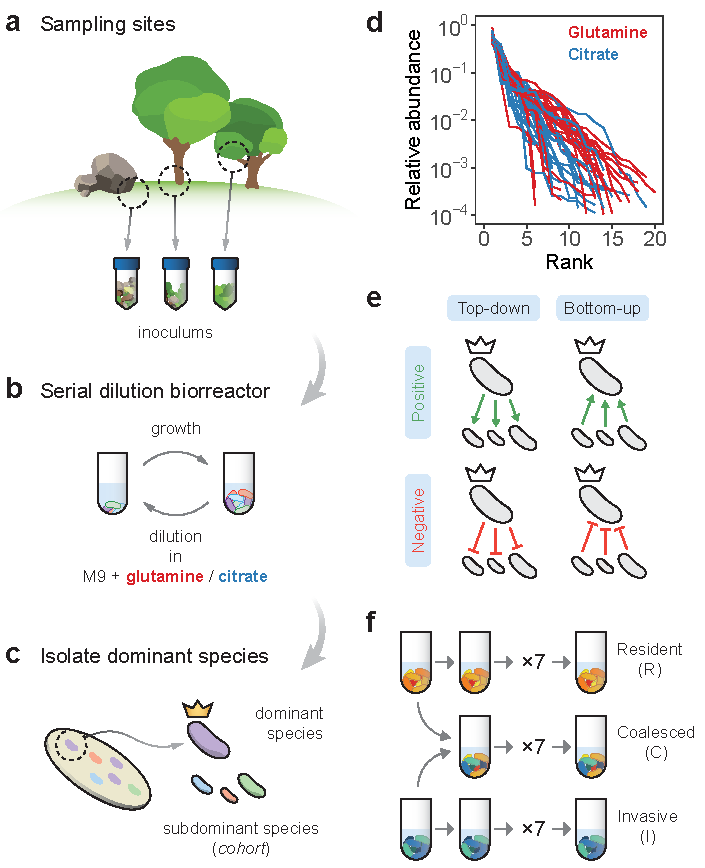
\includegraphics[width=0.8\linewidth,trim={4cm
        %     6.5cm 4cm 5.5cm}]{figs/final-layout/fig1}}
        \includegraphics[width=0.99\linewidth,keepaspectratio]{figs/fig1-crop-witharrows-compact}
	\internallinenumbers
	\caption[Inferring evolutionary trajectories using Cancer
        Progression Models.]{\textbf{Inferring evolutionary trajectories
            using Cancer Progression Models.} \textbf{A.} Example of a
          directed acyclic graph (DAG) of restrictions in the order of
          accumulation of mutations, analogous to the ones produced by
          most CPMs, such as CBN, MCCBN, OT, CAPRESE, and CAPRI. Given
          four driver genes (numbered 1 to 4), the DAG indicates the
          constraints in the order of accumulation of mutations
          (arrows). Here, a mutation in the 4th loci is conditioned to the
          2nd and 3rd ones having been previously mutated.  MHN uses a
          network to encode both promoting and inhibiting effects between
          pairs of events; the network could be identical to the one in A
          (meaning that mutations 2 and 3 have a promoting effect on
          mutation 4), but it could also include inhibiting effects; in
          contrast to DAGs of restrictions, MHNs do not denote
          deterministic dependencies.  \textbf{B.} Restrictions in the
          order of accumulation of mutations limit the amount of available
          evolutionary
          trajectories and stochastic dependencies change the
          probabilities of trajectories.  In this network, nodes represent
          different genotypes of four driver genes and edges connect those
          that are a single mutation away. Genotype names are assigned
          according to which genes are mutated (1) or not mutated
          (0). Without restrictions many mutational pathways are possible
          (any route through both solid and/or dashed edges, from left to
          right).  However, only a subset of genotypes satisfy the
          constraints in panel A (solid nodes); thus, only trajectories
          connecting these are predicted to be accessible pathways (solid
          edges). For example, given a specific genotype (1000, red node),
          restrictions in the mutational order limit the possible clones
          that can evolve from it consecutively after (red edges). With
          CBN, MCCBN, and OT, in addition to the set of accessible
          pathways, it is possible to obtain transition probabilities
          along the black lines.  Under the MHN model, as there are no
          deterministic dependencies, all transitions (to genotypes with
          one additional mutation) are possible, but transitions affected
          by inhibitory stochastic dependencies will have very low
          probability (in this simplified depiction they would be the gray
          lines) and those affected by promoting stochastic dependencies
          will have higher probability (black lines); MHN provides
          transition probabilities for all the lines in the figure.
          \textbf{C.}  Example of cancer progression with four driver
          genes under SSWM conditions. Progression towards the fitness
          maximum occurs through a defined sequence of parent-child
          genotypes, each one of them establishing as the most abundant
          rapidly after evolving. \textbf{D.} Example of cancer
          progression with four driver genes under conditions of no
          SSWM. Here, the sequence of parent-child genotypes from the
          wild-type with no driver mutations to the final one (i.e. the
          Line Of Descent or LOD) is: 0000 $\rightarrow$ 1000
          $\rightarrow$ 1010 $\rightarrow$ 1110. Notice that in the most
          general case, the ultimately fixated genotype need not be the
          one with all driver mutations (1111).  Some genotypes can be
          most abundant in the tumor during prolonged periods of time
          despite not being part of the LOD (0010, in green), and
          genotypes that do belong to the LOD may never be most abundant
          (1010, in blue). In all models and figures we do assume that
          there are no back mutations and that crossing valleys in the
          fitness landscape using a single multi-mutation step is not
          possible. }\label{fig:fig1}
\end{figure}



 
\begin{landscape}
  \begin{figure}[!h]
    \vspace*{-45pt}
%  \centering
\includegraphics[width=22.5cm,keepaspectratio]{figs/weighted-7-specific-no-split-01-sqrt-all_methods-js.pdf}
  \internallinenumbers
  \caption{\textbf{Linear mixed-effects model tree fitted to data from
      fitness landscapes with 7 loci, sample size of 4000 and uniform
      sampling.}  Internal nodes show the partitioning variables and the
    values that lead to each partition; light blue denotes the values or
    categories that lead down the left split and salmon the values or
    categories that lead down the right split (partitioning criteria are
    also shown in the edges leading down a node). Leaves or terminal nodes
    show (weighted) boxplots of the dependent variable for the
    observations that fall in that leave and, as label, the
    name of the node and the sample size (sum of weighted observations and
    \% of the total data set for the fit). The dot plots underneath the
    boxplots show the (weighted) mean JS for each method for that leave.}
  \label{fig:7_spec} \end{figure}
% \restoregeometry
\end{landscape}

\begin{figure}[!h]
  \centering
  %\includegraphics[width=15.5cm,keepaspectratio]{figs/boxplots-three-comps_all_datasets_combined.pdf}
  \includegraphics[width=15.5cm,keepaspectratio]{figs/biol_data_box_scatter.pdf}

  \caption{\textbf{Similarity between predictions of three pairs of
      methods for the 25 biological data sets.} For each data set, the JS
    divergence between the predictions of a pair of methods is represented in
    \textbf{A.}
    each of the three panels or \textbf{B.} each of the three axes. 
    Dots correspond to all genotypes
    for which we computed predictions, which are the genotypes observed in the
    samples, except for the genotype with all genes mutated if it was observed.
    In parentheses,
    after the data set, we indicate the total sample size (n) and number of genes (g).}
  
  \label{fig:biol_boxplots-3-comps} \end{figure}


\begin{figure}[!h]
  \centering
  \includegraphics[width=15.5cm,keepaspectratio]{figs/fraction_CE_TD_similar_all_datasets.pdf}

  \caption{\textbf{Percentage of genotypes with similar TD and similar CE
      predictions for the 25 biological data sets.} For each data set, the
    orange points show the percentage of genotypes in which predictions
    had both similar CE ($JS_{CBN, MHN} \le 0.0677$) and different CE-TD
    ($(1/2)\ (JS_{CBN, CBN\_td} + JS_{MHN, MHN\_td}) \ge 0.7$),  the
    blue dots those with similar TD ($JS_{CBN\_td, MHN\_td} \le 0.0677$)
    and different CE-TD, and the gray points the percentage of genotypes
    that had similar CE, similar TD, and different CE-TD. Values shown are the percentage relative to the
    total number of genotypes for which we computed predictions, which are
    the genotypes observed in the samples, except for the genotype with
    all genes mutated,
    if it was observed. In parentheses, after the data set, we indicate
    the total number of genotypes observed (GT).  % For a given data set, genotypes that have boot similar CE and
    % similar TD contribute to both counts.  Panels B) and C): scatter plots
    % of Similar TD and Similar CE, shown in panel A, against sample
    % size.
  }
  
  \label{fig:biol_freqs} \end{figure}


\end{document}






















%%%%%%%%%%%%%%%%%%%%%%%%%%%%%%%%%%%%%%%%%%%%%%%%%%%%%%%

%%% Old results stuff



% So: when we can achieve good performance depends crucially on
% balblaba. (Give one or two). And when we should used one type of method
% vs. other too (blablba)

% How is this relevant for real data sets, for which we know nothing of
% those characts? We have examined if this disyuntive could actually be
% relevant. And it is. Blabla.



% % \subsection{Results trees, II} \label{res2}

% % \begin{enumerate}
% % \item If prop local max is large, then a simple approach like TD works
% %   (CBN and MHN)
% %   % \begin{enumerate}
% %   % \item Fig 2 node 10 (2\% ), to lesser degree nodes 12, 13 (2 and 3
% %   %   perc.)
% %   % \item Suppl Fig 3: nodes 19 (and 20 and 21: 1 and 2 percent), node 16 (2
% %   %   perc) and 15 (1) and 22 (5 \% ) to lessser degree
% %   % \item Even in less than ideal situations that is the case. Suppl Fig 1:
% %   %   nodes 24 and 25 (with 1 and 5 \% )
% %   % \item Suppl Fig 2, nodes 18 and 22 (1 and 1 \% )
% %   % \item Lesser degree 16, 17, 23 (with 2, 1, 1,\% ): ehh??
% %   % \end{enumerate}
% % \item What about CE?
% %   \begin{enumerate}
% %   \item Cases where MHN is really the single best method are rare
% %   \item When CE can do well (JS < 0.2) most methods about equially good
% %     (except CAPRI), though CBN generally best (but recall simul scenarios
% %     might favor CBN). So when good CE performance, then pretty much any of
% %     the reasonable methods (all except CAPRI) will work. OT not the best,
% %     and MHN sometimes not best.
% %   \item CE is consistently gopod only in limited cases
% %     \begin{enumerate}
% %     \item Fig2: nodes 6, 7, 16, 20 (with 4, 1, 2, 6\% ); in node 16 MHN is
% %       poor
% %     \item Suppl Fig 1: Maybe node 6, 12, 16, 17 (with 1, 1, 2, 2\% data )
% %     \item Suppl Fig 2: nodes 10 and maybe 9 (sum of 2\% )
% %     \item Suppl Fig 3: node 23 (5\% ). OJO AQUI: probablemente escamotea
% %       que tenemos mezcla de buenos TD y buenos CE, como el nodo 19 en la
% %       figura del paper.
% %     \end{enumerate}
% %   \end{enumerate}
% % \end{enumerate}



% \subsection{Results: connect simuls-biol} \label{biol1}


% \begin{enumerate}
% \item If TD is good, the td methods are similar
% \item If CE is good, the CE methods are similar
% \item The converse is, of course, not true
% \item Particularly the case if TD and CE are very different.
% \item Refer to section ``Categorization of similarities between methods and
%   performance'' in suppl mat (i.e., use that info judiciously in the
%   paper, citing key numbers)
% \item Thus, we analyze biol data and focus on similar TD, similar CE,
%   dissimilar CE-TD: how often is this seen in the data?
% \end{enumerate}






% The fitness-landscape specific variables are

% - SSWM regime
% -  $\gamma$
% - (epistRSign)
% - numObservedPeaks

% - detection regime
% - sample\_size)

% - nMut
% - fitnessRank
% - propLocalMax

% - observedProp
% - diff\_obs\_prop

% epistRSign can flip which method is best: Node 11 in
% Fig.~\ref{S-fig:7_ALL}; smaller is better (also node 23 in the figure)

% numObservedPeaks can flip which method is best: Node 19 in
% Fig.~\ref{fig:7_spec}


% , ; notice that the effect of fitness landscape type
% is not always apparent in these trees, but three of the variables included
% in the fits, and that appear in the fitted trees, gamma, reciprocal sign
% epistasis, and number of observed peaks, 


% The fitted trees show (see supporting information, Figures \todo{blabla})
% show that \todo{blabla: sample size, detection regime}. The effect of
% fitness landscape type is not \todo{always, often} apparent in these
% trees, but three of the variables included in the fits, and that appear in
% the fitted trees, gamma, reciprocal sign epistasis, and number of observed
% peaks, allow to perfectly separate the RMF from the rest of the fitness
% landscape, and to separate most local maxima fitness landscapes from the
% representable ones (see figure \todo{gamma-rsign-obs-peaks-FL.pdf} in the
% supplementary material).


% The results for the tree fitted to seven genes, uniform, sample size =
% 4000, show \todo{blablabla}.



% Use the 7 genes, specific.

% number of peaks, ruggeddness of landscape matters: see node 28 vs. 29. Not
% unlike the pattern of 14 (here max fitness, so can only jump to end). node
% 28 also kinda matches node 21 in the 10 genes.  ode 28 is smooth, so it
% jumps to 7 mutations, it is often the single option. Note also node
% 15. And note that these cases add up to close to 8\% of observations


% Very obvious two different groups of methods, that, where it matters,
% either do a very good or a very bad job (with the other group doing a very
% bad or very good job)

% To prevent detection regime and sample size from hindering
% interpretation, we have fitted the models to the best performing
% conditions, sample size of 4000 and uniform detection regime.

% to prevent the effects of sample size and detection regime from
% obscuring key patterns.

% Our main objective is understanding the relevance of fitness
% landscape-specific and genotype-specific variables for on the quality of
% predictions. Thus, we have fitted the models to the best performing
% conditions, sample size of 4000 and uniform detection regime, to prevent
% the effects of sample size and detection regime from obscuring key
% patterns.



% The linear mixed-effects model trees fitted to the complete data sets for
% 7 and 10 genes showed that sample size and detection regime had a strong
% effect on performance (see Supplementary Material, Figures fig\_10\_ALL
% and fig\_7\_ALL), with better performance achieved under the uniform
% detection regime and with the largest sample size (4000) (see also Table
% tab\_minjs in Supplementary material); there are interactions,
% blablaba. We focus on something else.



% For both 7 and 10 genes, JS was smallest in the uniform detection regime
% with sample size of 4000 \todo{give numbers; do we even need this?}.



% \begin{figure}[!h]
%   \centering
%   \includegraphics[width=15.5cm,keepaspectratio]{figs/fraction_CE_TD_similar_all_datasets_combined.pdf}

%   \caption{\textbf{Percentage of genotypes with Similar TD or Similar CE
%       predictions for the 25 biological data sets.} A) For each data set,
%     the orange dots show the percentage of genotypes in which predictions
%     had both similar CE
%     ($(1/3) \ (JS_{CBN, MHN} + JS_{CBN, MCCBN} + JS_{MCCBN, MHN}) \le
%     0.0677$) and Different CE-TD
%     ($(1/2)\ (JS_{CBN, CBN\_td} + JS_{MHN, MHN\_td}) \ge 0.7$), and the
%     blue dots those with similar TD ($JS_{CBN\_td, MHN\_td} \le 0.0677$)
%     and Different CE-TD. Values shown are the percentage relative to the
%     total number of genotypes for which we computed predictions, which are
%     the genotypes observed in the samples, except for the last genotype,
%     if it was observed. In parentheses, after the data set, we indicate
%     the total number of genotypes observed (GT).  For a given data set, genotypes that have boot similar CE and
%     similar TD contribute to both counts.  Panels B) and C): scatter plots
%     of Similar TD and Similar CE, shown in panel A, against sample
%     size. }
  
%   \label{fig_biol_freqs} \end{figure}



%% FIXME Place in Suppl Mat
% \begin{figure}[!h]
%   \centering
  % \includegraphics[width=15.5cm,keepaspectratio]{figs/fraction_CE_TD_similar_all_datasets_sample_size.pdf}
  % \caption{\textbf{Percentage of genotypes with Similar TD or Similar CE
  %     predictions for the 24 biological data sets: relationship to sample size.} For each data set,
  %   the orange dots show the percentage of genotypes in which predictions had both similar CE
  %   ($(1/3) \ (JS_{CBN, MHN} + JS_{CBN, MCCBN} + JS_{MCCBN, MHN}) \le
  %   0.2$) and Different CE-TD ($(1/2)\  (JS_{CBN, CBN\_td} + JS_{MHN,
  %     MHN\_td}) \ge 0.6$), and the blue dots those with similar TD
  %   ($JS_{CBN\_td, MHN\_td} \le 0.2$) and Different CE-TD. Values shown
  %   are the percentage relative to the total number of genotypes for which we
  %   computed predictions, which are  the genotypes observed in the
  %   samples; the total number of genotypes observed is indicated to the
  %   right of the data set name as ``(n = x)''. For a given data set, the
  %   sum of the two numbers can be greater that 100, since genotypes that
  %   have boot similar CE and similar TD contribute to both counts.
  %    }
  
  % \label{fig_biol_freqs_sampsize} \end{figure}








%% From analyze-biol-data-3.R




% Figures \ref{S-fig:7_ALL} and \ref{S-fig:10_ALL} show the models
% fitted to all detection regimes and sample sizes; these figures showed the
% relevance of detection regime and sample size, with the smallest JS were
% generally achieved under the uniform detection regime and with the largest
% sample size (4000) (see also Supplementary material, Table
% \ref{S-tab_minjs} in section \nameref{S-suppl_minimal_js_ssize_det}).
% Moreover, there were interactions between detection regime and sample size
% on the one hand and genotype-specific and fitness landscape-specific
% variables. These interactions can make it harder to understand the
% relevance of fitness landscape-specific and genotype-specific variables on
% the quality of predictions, 


% . In the Supplementary Material
% (Fig.~\ref{S-fig:10_ALL}, section
% \ref{S-suppl-linear-mixed-model-results}) we show the results for 10
% genes.  These figures showed the relevance of detection regime and sample
% size, with the smallest JS were generally achieved under the uniform
% detection regime and with the largest sample size (4000) (see also
% Supplementary material, Table \ref{S-tab_minjs} in section
% \nameref{S-suppl_minimal_js_ssize_det}). Moreover, there are interactions
% between detection regime and sample size on the one hand and
% genotype-specific and fitness landscape-specific variables. These
% interactions can make it harder to understand the relevance of fitness
% landscape-specific and genotype-specific variables on the quality of
% predictions, which is one of the main objectives of this paper. Thus, we
% have fitted the linear mixed-effects model trees under the best performing
% conditions, sample size of 4000 and uniform detection regime, to isolate
% the effects of fitness landscape and genotype-specific variables; results
% are shown in Figure \ref{S-fig:7_spec} for fitness landscapes with seven
% genes, and in the Supplementary Material (Figure fig\_10\_spec) for
% fitness landscapes with 10 genes.

% The smallest JS were generally achieved under the uniform detection regime
% and with the largest sample size (4000) (see Supplementary material,
% ``Minimal JS for combinations of number of genes, sample size, and
% detection region'') %%Table tab\_minjs in
% a pattern that can also be observed in the linear
% mixed-effects model trees fitted to the complete data sets for 7 and 10
% genes (Supplementary Material, ``Linear mixed-effects model trees for
% complete data''). These figures also showed the presence of interactions
% between these two variables and other genotype-specific and fitness
% landscape-specific variables. These interactions can make it harder to
% understand the relevance of fitness landscape-specific and
% genotype-specific variables on the quality of predictions, which is one of
% the main objectives of this paper. Thus, we will focus below on models
% fitted under the best performing conditions, sample size of 4000 and
% uniform detection regime, to isolate the effects of fitness landscape and
% genotype-specific variables; results are shown in Figure \ref{S-fig:7_spec}
% for fitness landscapes with seven genes, and in the Supplementary Material
% (Figure fig\_10\_spec) for fitness landscapes with 10 genes.




%  of this same model nor
% in node 12 in Fig.~\ref{S-fig:10_ALL} since those nodes split genotypes landscapes
% that are not representable (). 



% Ojo: nodo 19 does not split con los de 1 peak, pero es 1 o 2, on the left!
% Some of these results are easy to understand. For example, in
% Fig.~\ref{fig:7_spec} the relevance of numObservedPeaks in node 19 for
% determining whether TD methods are better than their CE counterparts. Node
% 19 splits genotypes with 6 mutations (in fitness landscapes of 7
% genes). Now, if there is only peak, we are in a representable fitness
% landscape, and the next transition will necessarily be to the genotype
% with 7 mutations; the TD methods, that can predict that the genotype with
% 6 mutations is a local maximum will therefore fail. NOPE not that simple:
% a) this is 1 or 2 on the left, so not just representable; b) notice
% CAPRI's behavior.



% \idea{Ya no tengo nada claro que mostrar la figura que mostramos tenga
%   sentido. Podríamos mostrar solo la Suppl 1 y Suppl 2, en el main text.
%   No tengo claro que esté bien justificado (por que centrarse en los
%   mejores?) ni que ayude a clarificar la discusion. O lo ayudaría al
%   revés: mostar el Suppl Fig 1 en resultados, lo demças en suppl mat}

% \idea{La discusion podria ser muy distinta: complex interactions; SSWM,
%   rank, and other genotype specific matter. Done}



% They can be very
% different, but we still would need to choose. How? Using info we do not
% have about SSWM, fitness landscape, etc.



% Fig.~\ref{fig:biol_freqs} shows blablba \idea{add to that
%   plots those genotype where all three conditions are true; } So the CE
% can be similar, the TD can be similar: should we use them? When we observe
% similar CE and good performance depends on features we do not see; ditto
% for TD. And, even more dramatially, what if the same genotype shows both
% patterns?  They can be very different, but we still would need to
% choose. How? Using info we do not have about SSWM, fitness landscape, etc.



% since Fig.~\ref{fig:biol_freqs} based on the necessarily true conclusion
% that CBN and MHN can only both make correct predictions if both are making
% similar predictions, and similarly for CBN\_td and MHN\_td. Reversing the
% conditioning, however, does not guarantee a large improvement in
% performance.

% Using this simpleminded approach, we can in fact improve the
% performance, relative to baseline levels, if we condition on similar CE
% (or similar TD) but different CE-TD, but that improvement is rather modest
% \idea{blablaba ``Categorization of similarities between methods and
%   performance'' in suppl mat, and this is overestimate of performance,
%   etc, etc}. We can try to restrict the analysis to such
% conditions. Fig.~\ref{fig:biol_freqs} shows blablba \idea{add to that
%   plots those genotype where all three conditions are true; } So the CE
% can be similar, the TD can be similar: should we use them? When we observe
% similar CE and good performance depends on features we do not see; ditto
% for TD. And, even more dramatially, what if the same genotype shows both
% patterns?  They can be very different, but we still would need to
% choose. How? Using info we do not have about SSWM, fitness landscape, etc.


% \subsection{Results biol} \label{biol01}

% \begin{enumerate}
% \item In figure  \ref{fig:biol_freqs}
% \item Details for each data set (similarity CE, similarity TD, difference
%   CE-TD) in suppl mat (``Similarity of predictions for all genotypes for the biological
%   data sets'').
% \item Many cases where a large percentage genotypes very simlar TD or very
%   similar CE and very different CE to TD
% \item Wide variation among data sets
% \item Not related to sample size (panels B and C)
% \item Some of those preds could correspond to good predictions but telling
%   would require knowing more.
% \end{enumerate}




\section{Como hacer el conectar con datos biol: miscel, other ideas, what
  not to do, etc}
\label{sec:como-hacer-el}

Some options

\begin{enumerate}
\item Classify all output from simuls in four groups
  \begin{itemize}
  \item CE w.r.t. real approx 0, TD approx 1
  \item TD w.r.t. real approx 0, CE approx 1
  \item All $> 0.2$
  \item All $< 0.2$
  \end{itemize}
  \begin{itemize}
  \item But that sucks because we have a multi-class classification
    problem and that is a PITA with mixed effects
    models, etc.
\item Moreover, this
  would be circular thing (as it is based on previously looking at the
  data with the other trees). 
\item And of course we don't have anything similar with real data.

  \end{itemize}
\item Look at similarities between methods. What we didd with the other
  trees. That nothing came out, is it a result? Nope, since this is
  actually dealing with another issue. And it could be explored in much
  more detail. This ain't the point of the paper.
\item Focuse on some transitions/cases: like the genotype before
  last. E.g., node 19, 20, 21 in Fig 2. Pero eso es coger la cosas por los
  pelos. Compatre with node 23 in Suppl Fig 3. 
\item Try to do a principled search, over biological data, of regions with
  CE vs TD huge, within-CE small and within-TD small.

  Tghis requires defining things in a principled way. So the whole mess of
  a PCA if descriptive, PLS-like for predictive, etc. And we are back,
  like above, in another issue. Not what we are dealing with.
\item Focus on the key idea: choice of method/quality of predictions ought
  to depend on details of evol model etc that we ignore. Show how this
  matters. Show that it matters (Fig 2 of the paper) and show that there
  are many cases in biol data that likely fall there. \textbf{This is the
    connecting logic}.

  Emphasize: \textbf{we are not focusing on choice of single best method,
    just in seeing what is possible. Choice of best is a different
    question}.

  In results go over what is in \ref{res2}. Then, say:
  \begin{enumerate}
  \item If TD is good, the td methods are similar
  \item If CE is good, the CE methods are similar
  \item The converse is, of course, not true
  \item Refer to section ``Categorization of similarities between methods and
  performance'' in suppl mat (i.e., use that info judiciously in the
  paper, citing key numbers)
\item Now say: we will focus on cases in the biological data where the CEs
  are similar and the TDs are similar, as those can be good.
\item In the biological data, show statistics, for the data sets, of how
  often we have similar TD + dissimular CE-TD and similar CE + dissimilar
  CE-TD. Comment that ``choosing the best method and, thus, choosing
  predictions depends on key featuyres fo the evol model''. This is figure \ref{fig:biol_boxplots-3-comps}

  Show figure where it can be seen that we have used a whole bunch of data
  sets.

  We are done.


  \end{enumerate}


  \item Es tentador hacer más modelos de árboles con solo los datos
    simulados con
    buena predicción (JS $le 0.2$), y hacer modelo logístico para separar:
    ``los mejores son los TD'' vs.\ ``los mejores son los CE''. Pero esto:
    \begin{itemize}
    \item Es una pregunta distinta y el paper already too long
    \item Añade más tiempo de análisis.
    \item No está claro cómo se conecta con los datos biológicos.
    \item ¿Merece la pena?
    \end{itemize}


\item Es tentador hacer, con los datos simulados, una figura del tipo de
  \ref{fig:biol_freqs}. Dividiendo por type of landscape y por sampling
  type y quizas sample size. Pero:
  \begin{enumerate}
  \item Más tiempo análisis
  \item Alarga paper
  \item Delicate issue de los pesos
  \item Mejora la conexion pero no sé si merece la pena
  \end{enumerate}
    
  
\end{enumerate}

\idea{Do not forget to mention inherent variability of CBN (and MCCBN)
  which is very noticeable when relatively large number of variables, as
  has been noted before (Diaz-Uriarte and Vasallo, 2019; Hosseini et al.,
  2019). Ellaborate on this, etc, etc. Hosseini develops his strategy for
  this. With real data might one several runs for predicting genotye? etc,
etc. To be explored in further papers.}

\idea{Beware: we do not want anyone asking for cross-validatino of
  performance estimates! If they ask, we will say that outside of the
  scope, and a moot point anyway. Suppl mat tables present upper limits on
what is already modest performance}



Arriba en resultados explicar porqué uno se queda con cualquier genotipo
para el que hay rpedcciones de al menos 3. Uno de esos 3 siempre es MHN.











%%%%%%%%%%%%%%%%%%%%% Former biological data stuff




%  (note that being local maxima is often associated with having
% large relative fitness ---i.e., small fitness rank--- and local maxima
% genotypes are more common in fitness landscapes with a larger number of
% local fitness maxima)



% What those results emphasize, then, is that predicting if performance will
% be acceptable, and what method to use to achieve that performance, depends
% on features of the fitness landscape, the evolutionary process, and the
% genotype. This highlights the difficulties of interpreting the








The results from the simulated data have direct implications for the
interpretation of the application of these methods to biological data. As
Fig.~\ref{fig:biol_boxplots-3-comps} shows, there are often very large
differences in the predictions of a TD and a non-TD method (MHN vs.\
MHN\_td, right-most panel), something we could observe if we were dealing
with genotypes of types A) or B) above. But we have no solid grounds to
choose one method over the other, as that choice depends on information
about the evolutionary model and the genotype itself that we
ignore. Fig.~\ref{fig:biol_freqs} emphasizes this point: a tempting
approach when analyzing data would be to focus interpretation on genotypes
for which we see very dissimilar CE-TD predictions and at the same time
either similar TD or similar CE (or both).  This conditioning, by itself,
is unlikely to yield relevant improvements in performance (see Tables
\ref{S-tab:xtabs_td0} to \ref{S-tab:xtabs_ce1}). And it leaves unanswered
the question of which among the predictions that fulfill those similarity
conditions we should trust. The difficulty of this choice is even more
dramatic when the same genotype shows both large similarity within TD
methods, large similarity within CE methods, and large dissimilarity
between the CE and TD methods, as indicated by the gray points in
Fig.~\ref{fig:biol_freqs}: predictions between families of methods are
very different and yet choice of family of method would require fitness
landscape-specific and genotype-specific information.




\subsection{Analysis of biological data sets} \label{sec:biol-data}

\idea{algunas cosas de debajo repetir o enfatiza más en discusión y menos aquí}

% Do the above results matter for analysis of biological data? Yes they
% do.
When analyzing biological data, even if we do not know the true transition
probabilities, we can examine the consequences of assuming that we choose
one method when another method is the one that gives the best (or even
perfect) predictions. This is what we do in
Fig.~\ref{fig:biol_boxplots-3-comps}, where we use the four best
performing methods to illustrate the consequences of choosing the wrong
method. The left panel, for example, shows the difference in predictions
(measured using JS) if the method that gave perfect predictions were CBN
but we had used MHN (or viceversa).  As can be seen, for most data sets,
there is wide variability in the consequences of using the wrong method,
and often the difference in predictions is very large, specially if we use
a TD vs.\ a non-TD method (MHN vs.\ MHN\_td, right-most
panel).% And most of the time we have no
% solid grounds to choose one method over the other, as that choice depends
% on information about the evolutionary model and the genotype itself that
% we ignore.


% \idea{}The 25 biol data sets show ranges of variation
% comparable to those from the simulated data \idea{DO THIS PLOT for suppl
%   mat}.







\idea{algunas cosas de debajo mover a discusion: ``more dramatic'', blablablba}

% A naive approach might try to leverage on the similarity between methods, 
% as we have seen % :
% Fig.~\ref{fig:7_spec}, as well as Figures~\ref{S-fig:10_spec},
% \ref{S-fig:7_ALL} and \ref{S-fig:10_ALL}, indicate
We have seen, with the simulated data, that there is a sharp difference in
behavior of TD and CE methods when the best achievable performance is
good.  And necessarily CBN and MHN can only both make correct predictions
if both are making similar predictions; likewise, CBN\_td and MHN\_td can
only both make correct predictions if both are making similar prediction.
A simple approach could try to limit analyses to genotypes that show very
distinct CE-TD patterns and either  similar CE patterns, or similar
TD patterns. Note that conditioning in these similarity patterns could
bring at most very modest improvements in performance (see Tables
\ref{S-tab:xtabs_td0} to \ref{S-tab:xtabs_ce1}).
Fig.~\ref{fig:biol_freqs} shows the fraction of genotypes, for each data
set, that meet fairly stringent conditions of similarity either within the
CE methods (i.e., between CBN and MHN) or within the TD methods (i.e.,
between CBN\_td and MHN\_td). (See Supplementary Material, figures in
Section \ref{S-sm-indiv-biol-data-plots}, for similarity for each
individual genotype for each data set; note that these patterns are not
related to sample size ---see Fig.~\ref{S-fig:biol_freqs_sampsize}). There
is wide variation among biological data sets for the fraction of genotypes
that meet these criteria, but for several of the data sets, there are more
than 20\% of the genotypes that fall in either of these categories,
including genotypes for which all three criteria (dissimilar CE-TD,
similar TD, similar CE) are met.



% A naive approach might try to leverage on the similarity between methods, 
% as we have seen % :
% % Fig.~\ref{fig:7_spec}, as well as Figures~\ref{S-fig:10_spec},
% % \ref{S-fig:7_ALL} and \ref{S-fig:10_ALL}, indicate
% that there is a sharp
% difference in behavior of methods when the best achievable performance is
% good. And necessarily CBN and MHN can only both make correct predictions
% if both are making similar predictions; likewise, CBN\_td and MHN\_td can
% only both make correct predictions if both are making similar prediction.
% But, by itself, conditioning in these similarity patterns within CE
% methods and within TD methods could bring at most very modest improvements
% in performance (see Tables \ref{S-tab:xtabs_td0} to
% \ref{S-tab:xtabs_ce1}). Fig.~\ref{fig:biol_freqs} shows the fraction of
% genotypes, for each data set, that meet fairly stringent conditions of
% similarity either within the CE methods (i.e., between CBN and MHN) or
% within the TD methods (i.e., between CBN\_td and MHN\_td). (See
% Supplementary Material, figures in Section
% \ref{S-sm-indiv-biol-data-plots}, for similarity for each individual
% genotype for each data set; note that these patterns are not related to
% sample size ---see Fig.~\ref{S-fig:biol_freqs_sampsize}). There is wide
% variation among biological data sets, and for several of the data sets,
% there is a large fraction of genotypes with very simlar TD or very similar
% CE and very different CE to TD. Which among these predictions could we
% trust?  The difficulty of this choice is even more dramatic when the same
% genotype shows both large similarity within TD methods, large similarity
% within CE methods, and large dissimilarity between the CE and TD methods,
% as indicated by the gray points in Fig.~\ref{fig:biol_freqs}: predictions
% between families of methods are very different and yet choice of family of
% method would require fitness landscape-specific and genotype-specific
% information, as we have seen in Fig.~\ref{fig:7_spec}, as well as
% Figures~\ref{S-fig:10_spec}, \ref{S-fig:7_ALL} and \ref{S-fig:10_ALL}.









\subsubsection*{SSWM}

Deviations from SSWM are known to undermine the predictive power of CPMs \cite{diaz-uriarte2018,diaz-uriarte2019a}. The model underlying most CPMs seems to implicitly assume SSWM mainly for two reasons: \textit{a)} CPMs are powered with cross sectional data that do not undergo any deconvolution step (i.e. inference of clonal composition of the sequenced tumor), implying that a unique genotype\todo{``clone genotype"?} can be obtained from bulk sequencing, and \textit{b)} those observed clones are considered true steps in the path to tumor fixation, thus neglecting the possibility of tunneling effects. The two are true only if there is SSWM, in which case the most fit genotype at any given time is effectively the only one in the population and a direct ancestor of the ultimately fixated one. Even when CPMs specifically include error estimations (e.g. in Gerstrung et al., 2009\cite{Gerstung2009}), these typically refer to sequencing error but not necessarily to deviations from SSWM.




\iffalse
Most CPMs assume that cancer progresses under conditions of strong
selection and weak mutation (SSWM).\cite{hosseini2019a}\todo{I do not
find where Hosseini et al say that. Reword along:}
\idea{The model underlying most CPMs seems to
  implicitly assume SSWM: poorly written now, but a couple of key ideas:
  observed data are used directly, without any deconvolution step, which
  seems to indicate that even bulk sequencing can obtain a ``clone
  genotype''; this would only work if SSWM; and then those observed clone
  genotypes are considered true steps in the path to the maximum (i.e., no
  tunneling); note that the error included in models, e.g., Gerstung et
  al., 2009, is designed to capture sequencing error, but not necessarily
  deviations from SSWM ---slightly more subtle in MCCBN, though. Reword
  this properly, move stuff out to discussion, and leave here a simple
  sentence. One part of that sentence could be ``This assumption is rarely
  stated explicitly, but it is explicit in how \cite{hosseini2019a} use
  CBN for predicting tumor evolution.''  } \idea{Recheck MHN paper for
  SSWM}.
\fi

\idea{  One part of that sentence could be ``This assumption is rarely
  stated explicitly, but it is explicit in how \cite{hosseini2019a} use
  CBN for predicting tumor evolution.''  } \idea{Recheck MHN paper for
  SSWM}.





this number has an inverted U-shape with the
number of mutated loci (for a genotype $i$, the number of non-zero
$p_{i,j}$ is ${N}\choose{n + 1}$, where $n$ is the number of mutations of
the genotype and $N$ the total number of loci). 



When we are interested in predicting the complete evolutionary path the
only features that matter are global features.
 But when we want to make conditional, short-term
predictions, features of the genotypes for which we make the conditional
predictions can be as relevant as, or more relevant than, fitness
landscape-specific features \idea{citar banks y quizas otros}. This is a
noteworthy difference because it suggests that CPMs could be leveraged to
provide short-term predictions even when global, long-term predictions are
difficult because fitness landscape-specific assumptions are violated.


Our results indicate that,
were we to know a genotype can be a local maximum, specially if SSWM
holds, then we could make 


Los resultados de que a veces algunos tipos de métodos dan valores muy
similares enter sí, pero muy distintos a otros, no son solo cosa de las
simulaciones sino tb. en datos empírciso; ojo entonces con la
interpretación porque depende de factores que no conocemos.  \idea{plot el
  MHN vs MHN\_td para simulados?  sea como
  \ref{fig:biol_boxplots-3-comps}?}




\idea{remember that the local
maxima scenarios could slightly favor CBN, since the local maxima
landscapes are built as deviations from the CBN, and in part from OT/CAPRESE ).Also representable? What is the model for MHN?}




\idea{Null model no está. Either mention in results, when we mention
  results for number of mutations. Or mention here. I think that to keep
  ms short, null model figures should go in suppl mat, unless null model
  becomes a more important part of the ms.}


% \begin{figure}[H]
%   \centering
%   \fcolorbox{black}{white}{\includegraphics[width=0.8\linewidth,trim={4.5cm 10cm 4cm 9cm}]{figs/figexp}}
%   \internallinenumbers
%   \caption[Figure title]{\textbf{Figure title.} Figure caption. \idea{Esta
%     figura tapa texto encima}}
%   \label{figexp}
% \end{figure}




% The effects of the sampling and
% fitness landscape characteristics in predicting short-term evolution (as
% summarized in the linear mixed-effects trees (Fig.~\ref{fig:7_spec} and
% Supplementary Material Figs.~\ref{S-fig:10_spec}, ~\ref{S-fig:7_ALL},
% ~\ref{S-fig:10_ALL}) are, thus, not surprising. What is noteworthy is that
% local, genotype-specific features, i.e., features of the genotypes for
% which we make the conditional predictions, can be much more relevant than
% fitness landscape-specific features \idea{citar banks y quizas
%   otros}. These suggests that CPMs could be leveraged to provide
% short-term predictions even when global, long-term predictions are
% difficult: when we are interested in predicting the complete path
% evolutionary path, of course, the only features that matter are global
% features and these can often lead to poor performance
% \cite{diaz-uriarte2019a}. Our results here, however, indicate that good
% conditional predictions are possible even if fitness landscape-specific
% assumptions are violated.

% \idea{NO! Reword as}


% The effects of the sampling and
% fitness landscape characteristics in predicting short-term evolution (as
% summarized in the linear mixed-effects trees (Fig.~\ref{fig:7_spec} and
% Supplementary Material Figs.~\ref{S-fig:10_spec}, ~\ref{S-fig:7_ALL},
% ~\ref{S-fig:10_ALL}) are, thus, not surprising.





#####################   SSWM



it is widely accepted that intra-tumor heterogeneity is
common in cancer \cite{mcgranahan_clonal_2017, hinohara2019, zhao2016},
which can be partly due to deviations from SSWM arising from clonal
interference and stochastic tunneling
\cite{devisser_empirical_2014,szendro_predictability_2013,sniegowski_beneficial_2010};
for example, in multiple myeloma ``heteroeneoys clonal mixtures with
shifting predominant clones'' have been described
\cite[][p.~1067]{keats2012} %% could give example of Goto et al., 2018
                            %% lung cancer
suggesting the existence of non-SSWM regimes,
and stochastic tunneling in
cancer has, itself, been the focus of theoretical work
\cite[e.g.,][]{Ashcroft2015,wodarz_dynamics_2014}.
% deviations from SSWM and phenomena such as clonal
% interference and stochastic tunneling (due to rugged fitness landscapes
% where epistasis is common) are frequent
% \cite{devisser_empirical_2014}\todo{more refs; in fact, this is not a
%   reference about cancer}. \idea{search for refs of SSWM and tunneling in
%   cancer; there is one by Michor and see also the book by Wodarz and
%   komarova}.



it is widely accepted that intra-tumor heterogeneity is
common in cancer \cite{mcgranahan_clonal_2017, hinohara2019, zhao2016},
which can be partly due to deviations from SSWM arising from clonal
interference and stochastic tunneling
\cite{devisser_empirical_2014,szendro_predictability_2013,sniegowski_beneficial_2010};
for example, in multiple myeloma ``heteroeneoys clonal mixtures with
shifting predominant clones'' have been described
\cite[][p.~1067]{keats2012} %% could give example of Goto et al., 2018
                            %% lung cancer
suggesting the existence of non-SSWM regimes,
and stochastic tunneling in
cancer has, itself, been the focus of theoretical work
\cite[e.g.,][]{Ashcroft2015,wodarz_dynamics_2014}.
% deviations from SSWM and phenomena such as clonal
% interference and stochastic tunneling (due to rugged fitness landscapes
% where epistasis is common) are frequent
% \cite{devisser_empirical_2014}\todo{more refs; in fact, this is not a
%   reference about cancer}. \idea{search for refs of SSWM and tunneling in
%   cancer; there is one by Michor and see also the book by Wodarz and
%   komarova}.


When we move away from SSWM, multiple clones can coexist at significant
fractions for prolonged periods of time, and new higher-fitness clones can
evolve from low fitness parents that represented a minority of the
population. Genotypes with a large number of
mutations %high mutational load
can already be present at the time of sampling yet go undetected if their
relative abundance is small (figure
\ref{fig:fig1}D). % Deviations from SSWM
% are known to undermine the predictive power of CPMs
% \cite{diaz-uriarte2018,diaz-uriarte2019a}, as the model underlying most
% CPMs seems to assume SSWM (see Discussion). This assumption, however, is
% not always stated
% explicitly.
% , but it is explicit, for example, in Hosseini et al.'s
% \cite{hosseini2019a} use of CPMs for predicting tumor evolution (see
% \nameref{discussion}).



Widely accepted that ITH common in cancer \cite{mcgranahan_clonal_2017}
and there are examples that suggest presence of non-SSWM regimes
\cite{keats2012} with ``heteroeneoys clonal mixtures with shifting
predominant clones'' and stochastic tunneling has, itself, been the focus
of theoretical work \cite{Ashcroft2015}



\cite{bauer2015}: yeap, cite this for predict in
non-SSWM



###############################################################


%%% Local Variables:
%%% mode: latex
%%% TeX-master: t
%%% End:

